% ============================================================
%  MediPilot — Accenture Innovation Challenge 2026, Round II
%  Detailed Business Proposal | Team 01 BIT
%  Aditya Onam · Aditya Gupta · Varada Patel
%
%  House style shared with the Round I white paper and the
%  implementation README (docs/paper/implementation_readme.tex).
%  Every number in this document is traceable to a committed
%  artifact under docs/benchmarks/ or backend/model/artifacts/.
% ============================================================
\documentclass[10pt,a4paper,twocolumn]{article}

\usepackage[T1]{fontenc}
\usepackage[utf8]{inputenc}
\usepackage{newtxtext,newtxmath}
\usepackage{helvet}
\usepackage{microtype}

% ---------- Palette ----------
\usepackage[table,svgnames]{xcolor}
\definecolor{AccPurple}{HTML}{A100FF}
\definecolor{SecPurple}{HTML}{6F00B8}
\definecolor{DeepPurple}{HTML}{4B0082}
\definecolor{DarkPlum}{HTML}{24003D}
\definecolor{NearBlack}{HTML}{111111}
\definecolor{MedGray}{HTML}{666666}
\definecolor{CardBg}{HTML}{F7F7F7}
\definecolor{SoftGray}{HTML}{F2F2F2}
\definecolor{Border}{HTML}{E2E2E2}
\definecolor{White}{HTML}{FFFFFF}
\definecolor{TriRed}{HTML}{C0392B}
\definecolor{TriAmber}{HTML}{C98A17}
\definecolor{TriGreen}{HTML}{2E7D5B}

\usepackage[a4paper,top=1.9cm,bottom=2.0cm,left=1.8cm,right=1.8cm]{geometry}
\setlength{\columnsep}{0.72cm}

\usepackage{graphicx}
\usepackage{booktabs,array}
\usepackage{enumitem}
\usepackage[most]{tcolorbox}
\usepackage{titlesec}
\usepackage{fancyhdr}
\usepackage{lastpage}
\usepackage{caption}
% supertabular breaks a long table across COLUMNS (longtable cannot, in
% twocolumn); balance evens the two columns of the final page.
\usepackage{supertabular}
\usepackage{balance}
\usepackage{tikz}
\usepackage{pgfplots}
\pgfplotsset{compat=1.18}
\usetikzlibrary{positioning,calc,arrows.meta,fit,backgrounds,patterns}
\usepackage[colorlinks=true,linkcolor=SecPurple,urlcolor=SecPurple,citecolor=SecPurple,
  pdftitle={MediPilot: Detailed Business Proposal},
  pdfauthor={Aditya Onam, Aditya Gupta, Varada Patel}]{hyperref}

% ---------- Text ----------
\color{NearBlack}
\setlength{\parindent}{1em}
\setlength{\parskip}{0pt}
\linespread{1.02}
\raggedbottom
\renewcommand{\topfraction}{0.92}
\renewcommand{\textfraction}{0.06}
\renewcommand{\floatpagefraction}{0.80}
\setlength{\textfloatsep}{10pt plus 2pt minus 2pt}
\setlength{\dblfloatsep}{10pt plus 2pt minus 2pt}
\setlength{\dbltextfloatsep}{10pt plus 2pt minus 2pt}

% ---------- Headings ----------
\titleformat{\section}{\sffamily\bfseries\small\color{NearBlack}}
  {\textcolor{AccPurple}{\thesection}}{0.5em}{\MakeUppercase}
  [\vspace{-4pt}\textcolor{AccPurple}{\rule{\linewidth}{1pt}}]
\titlespacing*{\section}{0pt}{9pt}{4pt}
\titleformat{\subsection}{\sffamily\bfseries\footnotesize\color{SecPurple}}
  {\thesubsection}{0.5em}{}
\titlespacing*{\subsection}{0pt}{7pt}{2pt}

% ---------- Boxes ----------
\tcbset{mpbox/.style={enhanced,sharp corners=all,
  colback=CardBg,colframe=AccPurple,boxrule=0pt,leftrule=2.2pt,
  left=5pt,right=5pt,top=4pt,bottom=4pt,fontupper=\footnotesize}}
\tcbset{mpthesis/.style={enhanced,arc=2pt,
  colback=DarkPlum,colframe=DarkPlum,coltext=White,boxrule=0pt,
  left=6pt,right=6pt,top=5pt,bottom=5pt,fontupper=\footnotesize}}
\tcbset{mpcode/.style={enhanced,arc=1pt,
  colback=NearBlack,coltext=White,colframe=NearBlack,boxrule=0pt,
  left=5pt,right=5pt,top=4pt,bottom=4pt,fontupper=\ttfamily\scriptsize}}
\tcbset{mpwarn/.style={enhanced,sharp corners=all,
  colback=SoftGray,colframe=TriRed,boxrule=0pt,leftrule=2.2pt,
  left=5pt,right=5pt,top=4pt,bottom=4pt,fontupper=\footnotesize}}

\setlist[itemize]{leftmargin=1.1em,topsep=2pt,itemsep=1pt,parsep=0pt,
  label={\footnotesize\textcolor{AccPurple}{\textbullet}}}
\setlist[enumerate]{leftmargin=1.4em,topsep=2pt,itemsep=1pt,parsep=0pt}

\captionsetup{font={footnotesize,sf,color=MedGray},
  labelfont={bf,color=AccPurple},labelsep=period,skip=4pt}

% ---------- Furniture ----------
\pagestyle{fancy}\fancyhf{}\renewcommand{\headrulewidth}{0pt}
\fancyfoot[C]{\textcolor{Border}{\rule{\linewidth}{0.4pt}}\\[2pt]
  \sffamily\scriptsize\color{MedGray}%
  MediPilot \textbullet\ Business Proposal \textbullet\ Team 01 BIT\hfill
  \textcolor{AccPurple}{\thepage}\,/\,\pageref{LastPage}}

% ---------- Helpers ----------
\newcommand{\pth}[1]{\textcolor{SecPurple}{\texttt{#1}}}
\newcommand{\cm}[1]{\texttt{#1}}
\newcommand{\ix}[3]{{\sffamily\scriptsize\textcolor{AccPurple}{\bfseries #1}\ \ #2\ \dotfill\ p.\,\pageref{#3}}}
\newcommand{\pid}[1]{{\sffamily\bfseries\color{SecPurple}#1}}
\newcommand{\gpass}{{\sffamily\bfseries\scriptsize\color{TriGreen}pass}}
\newcommand{\gfail}{{\sffamily\bfseries\scriptsize\color{TriRed}FAIL}}

\begin{document}

% ======================= TITLE =======================
\twocolumn[{%
\vspace{-6mm}
\noindent\begin{minipage}[b]{0.74\textwidth}
  \raggedright\hyphenpenalty=10000\exhyphenpenalty=10000
  {\sffamily\scriptsize\color{AccPurple}\bfseries
   ACCENTURE INNOVATION CHALLENGE 2026 \ \textbullet\ \ ROUND II \ \textbullet\ \ PATIENTTRIAGE.AI}\\[5pt]
  {\sffamily\bfseries\LARGE\color{NearBlack}
   \textcolor{AccPurple}{Medi}Pilot: Detailed Business Proposal\\[2pt]
   Continuous Re-Triage for the Indian Emergency Department}
\end{minipage}\hfill
\begin{minipage}[b]{0.24\textwidth}
  \raggedleft
\includegraphics[height=22pt]{assets/accenture_logo.png}
\end{minipage}

\vspace{5pt}
\noindent\textcolor{AccPurple}{\rule{\textwidth}{1.4pt}}\\[-3pt]
\noindent\textcolor{Border}{\rule{\textwidth}{0.5pt}}

\vspace{5pt}
\noindent{\sffamily\footnotesize\bfseries
  Aditya Onam \quad Aditya Gupta \quad Varada Patel}\\[1pt]
\noindent{\sffamily\scriptsize\color{MedGray}
  Team 01 BIT \ \textbullet\ \ Indian Institute of Technology Patna \ \textbullet\ \ August 2026}

\vspace{7pt}
\begin{tcolorbox}[mpbox,colback=White,leftrule=0pt,left=0pt,right=0pt,top=2pt,bottom=2pt]
{\sffamily\scriptsize\bfseries\color{AccPurple}EXECUTIVE SUMMARY}\\[2pt]
\footnotesize
Emergency department crowding kills through a structural defect rather than individual error:
acuity is assigned once, at arrival, and the queue that results is static while the patient's
physiology is not. \textbf{MediPilot is a continuous re-triage platform built on one architectural
invariant --- the system may raise a waiting patient's priority autonomously, and may never lower
it below a human-assigned level.} Escalation costs one nurse assessment; de-escalation can cost a
life, so it stays with a human.

This document is the Round~II business proposal, and it is backed by a working prototype rather
than a specification. Seven clinical surfaces run end to end over a 20-patient synthetic corpus
that covers every case the brief mandates --- an ambiguous epigastric presentation, a
paediatric/geriatric pair at the same fever, a zero-history first attendance, a 3$\times$ surge, a
clinician override with its audit record, and an out-of-distribution patient the system refuses to
score. Six age strata are calibrated separately, because a single adult-calibrated model is a
silent safety risk: our own corpus shows a 3-year-old at 38.7\,\textdegree C with a heart rate of
138 that is \emph{normal for age} and would read as severe tachycardia on an adult scale.

We report evaluation honestly, including where it is unflattering. A four-model Risk Engine
bake-off on a freshly generated 20{,}000-patient held-out split shows the shipped
gradient-boosted model leading on discrimination (AUPRC 0.164) and calibration (ECE 0.011) and
being the only candidate to hold conformal coverage at or above 90\%. It also shows that
\emph{no} learned model reliably beats the hand-coded rule card at tight operating points --- which
is precisely why the rule card remains the floor of the architecture rather than a fallback we
hope never to use. On the perception side, a ten-candidate LLM structurer bake-off gives
\cm{gpt-oss-120b} an F1 of 0.962 with zero red flags missed against 0.510 and twelve missed for
the rule baseline, and a twelve-backend ASR bake-off selects the transcription path on measured
word error rate rather than on a vendor claim.

The commercial wedge is deliberately narrow: ship the deterioration-while-waiting module alone. It
carries the highest clinical value and the lowest regulatory exposure, because it never assigns an
initial acuity --- it only watches a queue a human already ordered.

\vspace{3pt}
{\sffamily\scriptsize\color{MedGray}\textbf{\color{NearBlack}Jurisdiction:}\; India --- DPDP Act 2023, ABDM consent framework, CDSCO SaMD pathway. \textbf{\color{NearBlack}Status:}\; working prototype on synthetic data; no clinical claim is made.}
\end{tcolorbox}

\vspace{5pt}
\begin{tcolorbox}[mpbox,colback=CardBg]
{\sffamily\scriptsize\bfseries\color{AccPurple}INDEX}\\[3pt]
\begin{tabular}{@{}p{5.15cm}p{5.15cm}p{5.15cm}@{}}
\ix{1}{Problem Framing}{sec:problem}        & \ix{5}{Data Strategy \& Limits}{sec:data}   & \ix{9}{Business Case \& Impact}{sec:business}\\[2pt]
\ix{2}{Solution Design}{sec:solution}       & \ix{6}{Testing \& Evaluation}{sec:eval}     & \ix{10}{Scalability}{sec:scale}\\[2pt]
\ix{3}{The Working Prototype}{sec:proto}    & \ix{7}{Target Users \& Adoption}{sec:users} & \ix{11}{Phased Roadmap}{sec:roadmap}\\[2pt]
\ix{4}{Age \& Site Calibration}{sec:calib}  & \ix{8}{Data Protection}{sec:reg}            & \ix{12}{Risks \& Mitigations}{sec:risk}\\
\end{tabular}
\end{tcolorbox}
\vspace{4pt}
}]

% ======================= 1. PROBLEM =======================
\section{Problem Framing}
\label{sec:problem}

\subsection{The defect is structural, not human}
The danger of an ED waiting room is not that patients arrive critically ill. It is that they
\emph{become} critically ill after being assigned a low priority, and no mechanism exists to
notice. A patient with mild chest discomfort receives a Yellow and sits down; twenty minutes later
they are hemodynamically unstable; the triage nurse is by then registering three new arrivals.

This is the \textbf{single-point assessment model}, and its failure rate is a property of the
process rather than of any clinician in it.

\begin{center}\footnotesize\sffamily
\begin{tabular}{@{}p{1.35cm}p{6.45cm}@{}}
\toprule
\rowcolor{AccPurple!10}
\textbf{Figure} & \textbf{What it measures}\\
\midrule
\textbf{32.2\%} & of US ED visits are mistriaged under ESI --- roughly one nurse label in three\\
\addlinespace[2pt]
\textbf{0.63} & AUC of the Epic Sepsis Model in external validation over 38{,}455 hospitalisations, against a marketed 0.76--0.83\\
\addlinespace[2pt]
\textbf{33\%} & its sensitivity: two of every three sepsis cases missed, while deployed at hundreds of US hospitals\\
\addlinespace[2pt]
\textbf{109} & alerts raised per true positive it did find --- the alert-fatigue failure mode\\
\addlinespace[2pt]
\textbf{11.7\%} / \textbf{3.6\%} & occult hypoxaemia, Black vs White patients, on pulse oximetry; 17\% vs 6.2\% in the multicentre cohort\\
\addlinespace[2pt]
\textbf{100--500} & ED visits per day this must serve, per the brief\\
\addlinespace[2pt]
\textbf{$\sim$50\%} & of arrivals carry any prior record at all\\
\bottomrule
\end{tabular}
\end{center}

\vspace{3pt}
Two of those numbers shape this entire proposal. The Epic Sepsis Model did not fail through
carelessness; it failed because it learned \emph{clinician suspicion} --- antibiotic-order timing ---
rather than physiology, and so detected the very process it was meant to augment. That is a
leakage failure, and \S\ref{sec:solution} gives the mechanism that makes it structurally impossible
here rather than merely discouraged. The oximetry figures are why a normal SpO\textsubscript{2}
carries no de-escalation authority anywhere in this system.

India had no nationally standardised ED triage protocol before the AIIMS Triage Protocol --- a
three-tier Red/Yellow/Green system since adopted by AIIMS Bhubaneswar, CMC Vellore, GTB Delhi and
the Kerala DHS. Most Indian EDs are staffed by generalists rather than emergency-medicine
specialists, so any workable system must run in a district hospital with one physician and one
nurse as reliably as in a tertiary centre.

\subsection{What the prototype already measures}
Three numbers from our own instrumentation frame the rest of this document. On the 20-patient
corpus, continuous five-minute re-scoring reaches the Yellow threshold a mean of \textbf{21.6
minutes} earlier than the next scheduled physical re-measurement would, and up to 55 minutes
earlier in individual cases (Fig.~\ref{fig:headstart}). The risk engine itself decides in
\textbf{3\,ms} at p50, p99 8\,ms (Fig.~\ref{fig:latency}). And the chosen structurer misses
\textbf{zero} red flags across a deliberately adversarial evaluation set, against twelve for the
deterministic baseline beneath it (Fig.~\ref{fig:slices}).

\begin{tcolorbox}[mpthesis]
\textbf{The contribution is not a better score. It is a better contract.} A machine that is
allowed to raise an alarm on its own, is never allowed to lower one, abstains out loud when it does
not know, and is evaluated on the patients it misses rather than on the average it gets right.
\end{tcolorbox}

\subsection{The seven complexities, and our answer to each}
The brief names seven real-world complexities. We treat them as design constraints rather than
caveats, and each maps to a mechanism that exists in the prototype.

\begin{center}\footnotesize\sffamily
\begin{tabular}{@{}p{2.35cm}p{5.45cm}@{}}
\toprule
\rowcolor{AccPurple!10}
\textbf{Complexity} & \textbf{Mechanism in the prototype}\\
\midrule
Ambiguous / under-reported symptoms &
Conformal abstention: the system returns an acuity \emph{set}, and when the set is wide it
declines and routes to a human (\pid{P-04}, \pid{P-08}). Reliability flags capture stoic
presentation and communication barriers (\pid{P-03}, \pid{P-16}, \pid{P-18})\\
\addlinespace[2pt]
Age-varying thresholds &
Six strata, each with its own normal ranges, its own isotonic calibration, its own conformal
quantile and its own decision threshold (\S\ref{sec:calib})\\
\addlinespace[2pt]
Uneven data at intake &
Train-time modality dropout at 40\%, so the model must produce a usable estimate from a snapshot;
zero-history is a first-class path (\pid{P-07})\\
\addlinespace[2pt]
Seconds to decide, and explainable &
One card: band, two strongest supporting factors, one opposing factor, and a confidence band. The
opposing factor is a deliberate falsification target\\
\addlinespace[2pt]
Asymmetric costs &
Cost ratio $R$ enters training as an asymmetric loss and sets the threshold, so objective and
operating point agree rather than being reconciled afterwards\\
\addlinespace[2pt]
Hospitals differ &
Every clinical knob is YAML, signed off per site; arrival rate, cadences, red flags and $R$ are
site parameters (\S\ref{sec:scale})\\
\addlinespace[2pt]
Accountability \& liability &
Override is a first-class route, not an escape hatch; every decision and reversal lands in a
SHA-256 hash-chained ledger (\S\ref{sec:reg})\\
\bottomrule
\end{tabular}
\end{center}

% ======================= 2. SOLUTION =======================
\section{Solution Design}
\label{sec:solution}

\begin{figure*}[p]
  \centering
  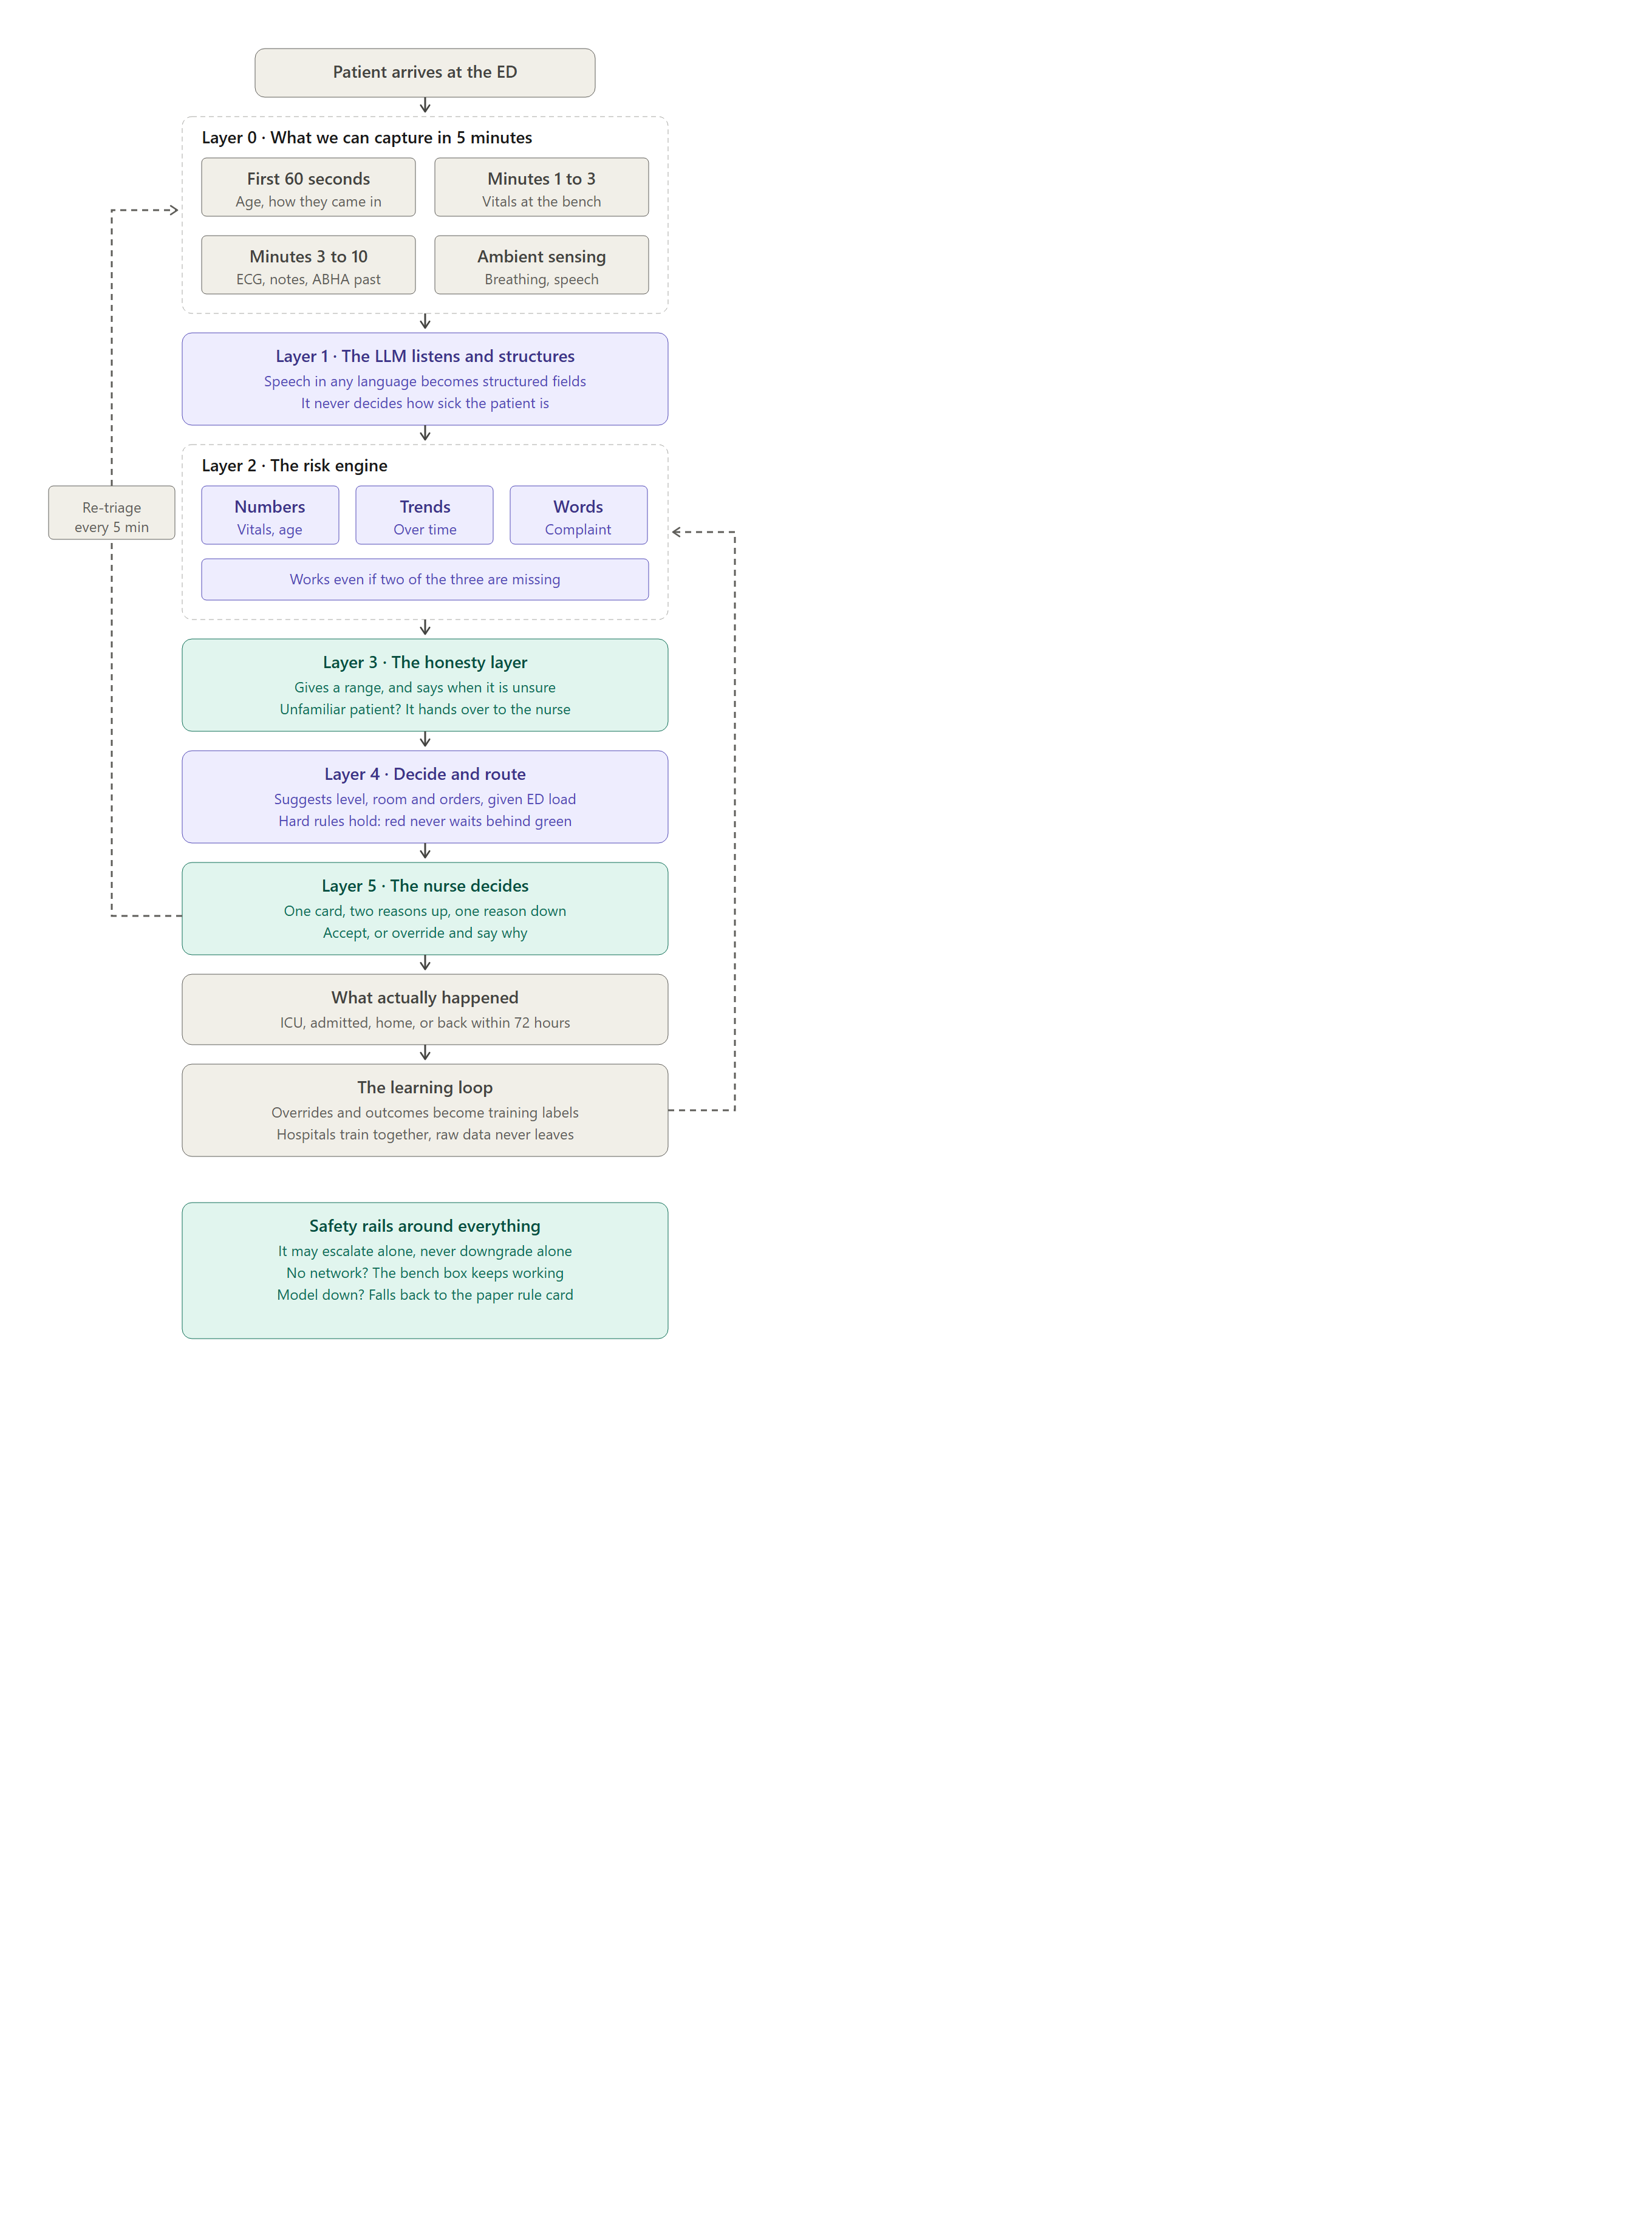
\includegraphics[trim=59 1463 1488 59,clip,height=0.86\textheight]{../diagrams/01-full-architecture.png}
  \caption{The six-layer pipeline and its two feedback loops. Layer~1 (the language model) may only
  structure speech --- it never decides how sick the patient is. Layer~2 fuses numbers, trends and
  words and works even if two of the three are missing. Layer~3 is permitted to say it does not
  know. The dashed return on the left is the five-minute re-triage loop that makes the corridor
  observed; the dashed return on the right is the learning loop, in which overrides and outcomes
  become training labels.}
  \label{fig:arch}
\end{figure*}

\subsection{One invariant, propagated through six layers}
MediPilot is a six-layer pipeline closed by two feedback loops (Fig.~\ref{fig:arch}). The
asymmetry is not a policy setting anywhere in it --- it is an architectural constraint. An attempt
to lower a band without an attached human action raises
\cm{AsymmetricAutonomyViolation} on the code path.

Formally, escalation is optimal when $c_{\text{FN}}\,p \ge c_{\text{FP}}(1-p)$, giving the
operating threshold
\[
p^{*} \;=\; \frac{c_{\text{FP}}}{c_{\text{FP}}+c_{\text{FN}}} \;=\; \frac{1}{1+R},
\qquad R = \frac{c_{\text{FN}}}{c_{\text{FP}}}.
\]
$R$ is a \textbf{per-hospital configurable parameter} set by clinical leadership at deployment, not
a global constant chosen by a vendor. The shipped artifact solves $R_{\text{yellow}}=12.2$ and
$R_{\text{red}}=5.8$ against an under-triage budget, giving thresholds $p^{*}_{\text{yellow}}=0.076$
and $p^{*}_{\text{red}}=0.147$.

\subsection{Data strategy --- weighing inputs that are never complete}
Inputs arrive in three windows with sharply different availability, and every field is registered
with its earliest availability time and a leakage class before it may be used at all.
\pth{config/feature\_registry.yaml} classifies each field \cm{SAFE}, \cm{CONDITIONAL} or
\cm{PROHIBITED} and \textbf{fails closed}: an unregistered name is treated as \cm{PROHIBITED}, so
adding a field without classifying it breaks the build. This is the mechanism that prevents the
failure that broke the Epic Sepsis Model, which learned \emph{clinician suspicion} (antibiotic
order timing) rather than physiology and scored AUC 0.63 at 33\% sensitivity in external
validation.

Operational context --- census, boarding count, staff on shift, bed availability --- is ingested by
the routing layer \emph{only}, and is explicitly excluded from the risk layers. Physiologic risk is
therefore never a function of how busy the department is.

The 59 features are six per vital: value, per-stratum $z$-score, reading age in minutes, slope per
hour, 30-minute delta, and a count of readings. That trend block is what makes
deterioration-while-waiting visible at all; a snapshot model cannot see a trajectory.

\subsection{Decision model --- hybrid, not a choice between rules and ML}
The brief offers rules, ML, or a hybrid. We use a strict hybrid with a fixed precedence, and the
deterministic layer wins:

\begin{center}\footnotesize\sffamily
\begin{tabular}{@{}p{0.6cm}p{7.2cm}@{}}
\toprule
\rowcolor{AccPurple!10}
\textbf{\#} & \textbf{Stage --- and who may overrule whom}\\
\midrule
1 & Stratum resolution from age\\
2 & Vital freshness --- stale readings are discounted at 2$\times$ cadence, treated as missing at 3$\times$\\
3 & \textbf{Deterministic red flags fire first} --- eight observations, each mapping straight to Red, overridable only by a clinician\\
4 & Vital thresholds, per stratum\\
5 & Raw ML risk\\
6 & Per-stratum isotonic calibration\\
7 & Asymmetric reliability weighting\\
8 & Conformal uncertainty\\
9 & \cm{ScoreObject} \emph{or} \cm{AbstentionObject} --- never a partial object\\
\bottomrule
\end{tabular}
\end{center}

\vspace{3pt}
Uncertainty is represented three ways, and all three are visible to the nurse. Isotonic calibration
makes the number mean what it says at that site. Mondrian split-conformal prediction
($\alpha=0.10$) returns an acuity \emph{set} with a formal coverage guarantee held separately
within each stratum. And an out-of-distribution gate routes unfamiliar patients to manual
assessment with an explanatory note. \textbf{The interface enforces this}: \cm{AcuityCard} throws
if asked to render a score without a confidence band, so a bare number cannot reach a screen even
by mistake.

\begin{figure*}[p]
  \centering
  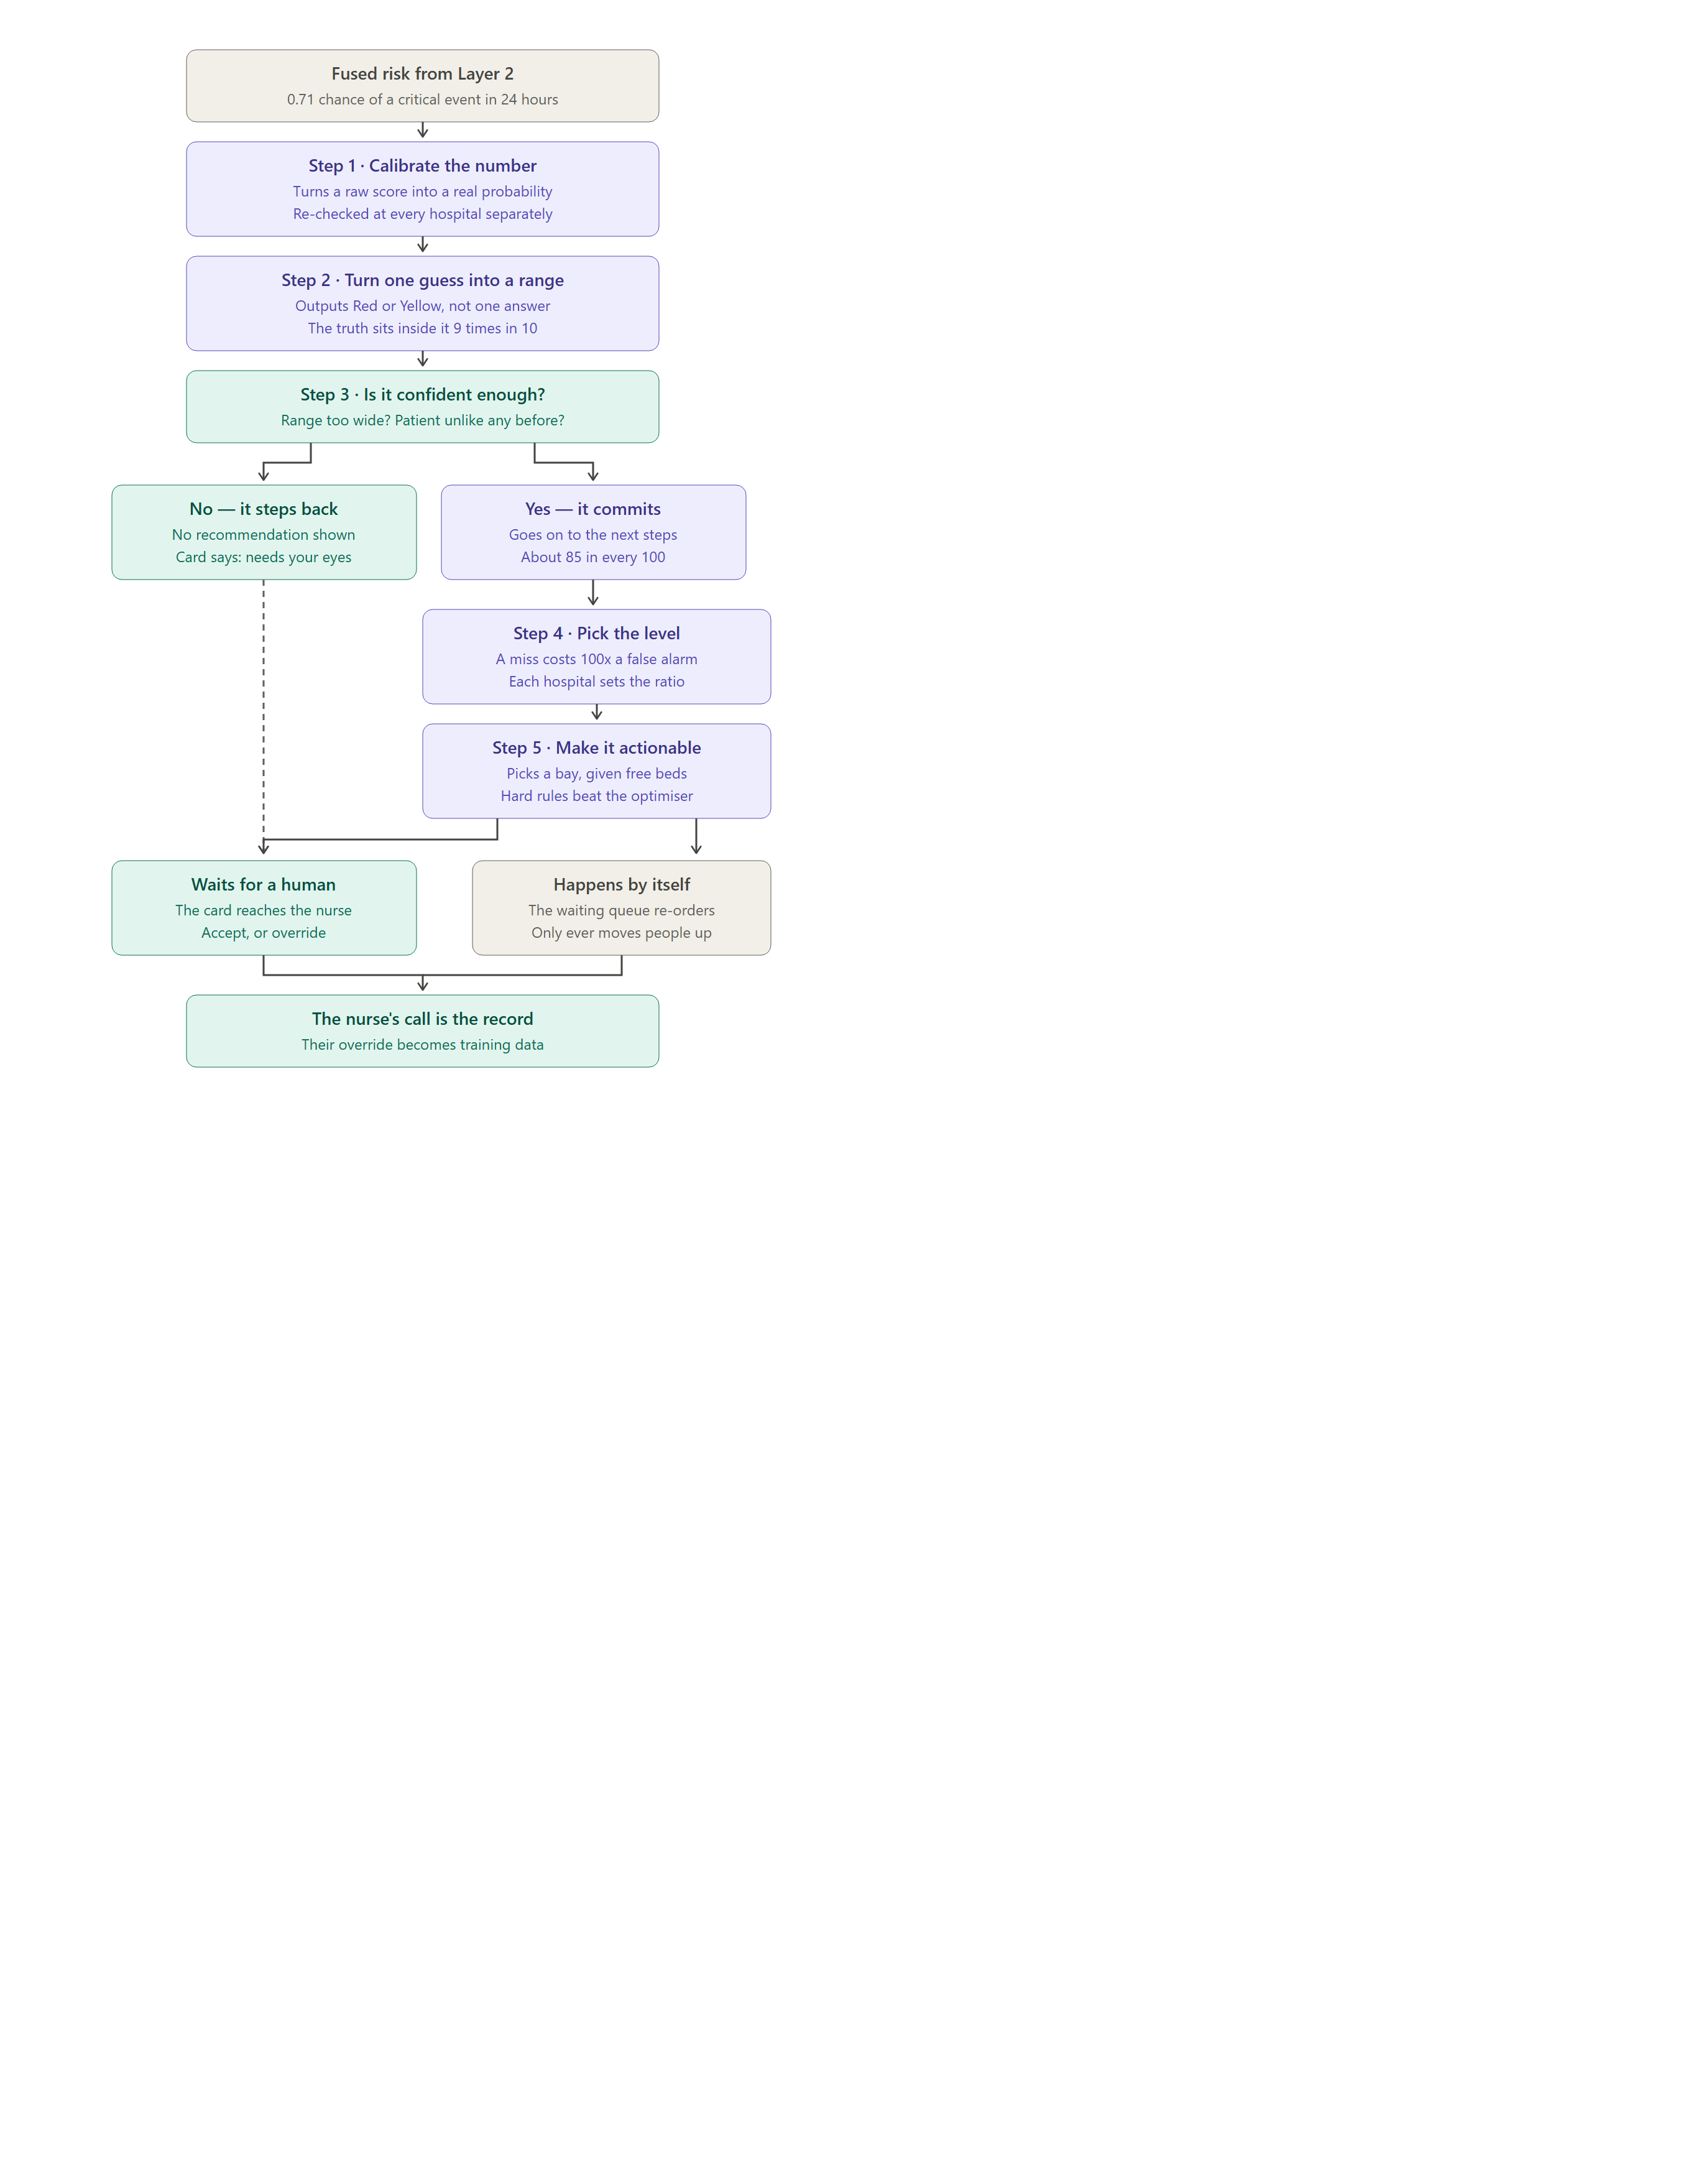
\includegraphics[trim=159 1775 1459 59,clip,height=0.85\textheight]{../diagrams/02-post-risk-engine-decision-path.png}
  \caption{The decision path in depth, from a fused risk number to a band on the board. Read it as
  four gates in series. \textbf{Step~1} turns a raw score into a probability that means what it says,
  re-checked at every hospital separately --- what \S\ref{sec:calib} calls per-site calibration.
  \textbf{Step~2} replaces the point estimate with a range that contains the truth nine times in
  ten. \textbf{Step~3} is the gate most systems omit: an explicit confidence check that may
  \emph{step back entirely}, showing no recommendation and routing the patient to a human. Only past
  that gate does the system pick a level --- and the split at the bottom is the invariant made
  visible: the queue re-orders by itself but only ever moves people \emph{up}, while anything that
  could lower a patient waits for a person. The nurse's call, not the model's, becomes the record,
  and therefore becomes the training data.}
  \label{fig:decisionpath}
\end{figure*}

\subsection{The decision path in depth}
Fig.~\ref{fig:decisionpath} expands stages 5--9 of the table above into the flow a single patient
actually takes. Two properties are worth naming because they are unusual. First, \textbf{abstention
is a terminal state, not an error} --- there is a path through this system that ends in "no
recommendation", drawn as a first-class outcome rather than an exception branch. Second,
\textbf{the two bottom boxes carry different authority}: "happens by itself" is the autonomous
escalation lane and is one-directional by construction, while "waits for a human" is everything
else. No arrow in that diagram moves a patient down without passing through a person.

\subsection{Workflow --- the moment, the override, the surge}
\emph{In the moment.} The nurse speaks normally; the system fills the form and reads the vitals
back so she can correct them before they commit. It never announces a level out loud where patients
can hear, and the hall speaker calls token numbers only --- never names or conditions.

\emph{The override.} One touch from every surface showing a band. The dialog captures a reason code
from a fixed list plus free text, because a fixed list never covers everything. The record fixes
\cm{inputs\_hash} so the decision is reproducible and \cm{factors\_shown} so the card as displayed
is preserved.

\emph{The surge.} Detected at 3$\times$ the site's normal arrival rate over a 20-minute rolling
window; exited below 2$\times$. Yellow re-measurement stretches 30$\rightarrow$45 minutes and Green
60$\rightarrow$90. \textbf{Red never stretches.} Three actions are forbidden under any load and
raise \cm{SurgeViolation} rather than being discouraged: raising $R$ to quieten alarms, resolving
an abstention by guessing, and de-escalating anyone to free capacity. Alerts are ranked by
$\text{risk}\times\text{minutes waiting}$ and are never suppressed.

\subsection{Safety-first defaults and the waiting loop}
Two clocks run per patient: re-score (model) and re-measure (physical). The brief requires
monitoring of the waiting queue, and this is the module that does it.

\begin{center}\footnotesize\sffamily
\begin{tabular}{@{}p{1.32cm}p{1.12cm}p{1.18cm}p{3.28cm}@{}}
\toprule
\rowcolor{AccPurple!10}
\textbf{Band} & \textbf{Re-score} & \textbf{Re-measure} & \textbf{Wait ceiling and breach action}\\
\midrule
Red & 1 min & 5 min & should not be waiting; pages a senior clinician at 5 min\\
\addlinespace[2pt]
Yellow & 5 min & 30 min & 60 min $\rightarrow$ forced re-measurement; escalates to Red if not done in 15 min\\
\addlinespace[2pt]
Green & 5 min & 60 min & 120 min $\rightarrow$ re-measure + wellbeing contact; two consecutive missed rechecks escalate to Yellow\\
\addlinespace[2pt]
Abstained & 5 min & on human review only & 15 min unreviewed $\rightarrow$ breach. Floor band is Yellow: an abstained patient is never Green\\
\bottomrule
\end{tabular}
\end{center}

\vspace{3pt}
Recheck trust is tiered, which matters in an Indian ED where families participate in care. A
recheck station or nurse can close any band. An accompanying family member can close a Green only,
and doing so raises a flag for staff. Patient self-service can \emph{escalate} but can never
de-escalate and can never satisfy a recheck.

% ======================= 3. PROTOTYPE =======================
\section{The Working Prototype}
\label{sec:proto}

\subsection{Against the brief's minimum expectations}
\begin{center}\footnotesize\sffamily
\begin{tabular}{@{}p{3.55cm}p{4.25cm}@{}}
\toprule
\rowcolor{AccPurple!10}
\textbf{Required} & \textbf{Delivered}\\
\midrule
Scoring on 15--20 simulated records & \textbf{20} deterministic records, \pid{P-01}--\pid{P-20}, seed 42\\
\addlinespace[2pt]
$\ge$1 ambiguous presentation & \pid{P-04} epigastric pain: gastritis vs inferior MI\\
\addlinespace[2pt]
$\ge$1 paediatric \emph{or} geriatric & \textbf{7} across five non-adult strata; \pid{P-02}/\pid{P-03} are the brief's own 38.5\,\textdegree C pair\\
\addlinespace[2pt]
$\ge$1 zero-history patient & \pid{P-07}, first attendance, no prior record\\
\addlinespace[2pt]
3$\times$ surge behaviour & \pid{P-10} under surge load; policy in \pth{surge\_policy.yaml}\\
\addlinespace[2pt]
No score without confidence & Enforced in the component, not by convention\\
\addlinespace[2pt]
$\ge$1 clinician override, logged & \pid{P-09}, 19-field hash-chained record\\
\bottomrule
\end{tabular}
\end{center}

\subsection{The 20-patient corpus}
Table~\ref{tab:corpus} is the whole corpus. \pid{P-01}--\pid{P-10} map to the acceptance cases in
the brief; \pid{P-11}--\pid{P-20} broaden stratum and condition coverage. Shaded rows are the cases
the brief names explicitly.

\begin{table*}[t]
\centering\footnotesize\sffamily
\caption{The 20-patient demonstration corpus (\pth{backend/data/corpus\_20.json}, seed 42,
deterministic). Shaded rows are the presentations the brief mandates. Every record carries a full
37-step vital trajectory from T=0 to T=180 minutes at 5-minute intervals, so deterioration is
replayable rather than asserted.}
\label{tab:corpus}
\begin{tabular}{@{}llllp{7.4cm}@{}}
\toprule
\rowcolor{AccPurple!10}
\textbf{ID} & \textbf{Age} & \textbf{Stratum} & \textbf{Case} & \textbf{What it is there to prove}\\
\midrule
\rowcolor{AccPurple!7}
P-01 & 42 y & adult & deteriorates while waiting & The core claim. Yellow at arrival, autonomously escalated partway through the wait\\
\rowcolor{AccPurple!7}
P-02 & 3 y & child & paediatric fever pair & 38.7\,\textdegree C, HR 138, RR 33 --- normal-for-age HR that an adult scale reads as severe tachycardia\\
\rowcolor{AccPurple!7}
P-03 & 75 y & geriatric & geriatric fever pair & 38.1\,\textdegree C, HR 68 --- unremarkable rate, but RR 22.9 and SpO$_2$ 93.5 are both out of range for age. Stoic presentation flagged\\
\rowcolor{AccPurple!7}
P-04 & 55 y & adult & ambiguous epigastric pain & Gastritis vs inferior MI. The ambiguous presentation the brief requires\\
P-05 & 35 y & adult & SpO$_2$ device bias & Dark skin, SpO$_2$ reads 96\%, patient distressed. A normal reading carries \emph{no} de-escalation authority\\
P-06 & 48 y & adult & stale vitals (3 h) & Freshness decay: beyond 3$\times$ cadence the reading is treated as missing, not as reassurance\\
\rowcolor{AccPurple!7}
P-07 & 38 y & adult & zero history & First attendance, nothing on file beyond what is observed now\\
\rowcolor{AccPurple!7}
P-08 & 50 y & adult & OOD abstention & Unusual vital combination. The system declines to score and says so\\
\rowcolor{AccPurple!7}
P-09 & 62 y & adult & nurse override & Yellow$\rightarrow$Red on a physical finding the system could not see. Produces the audit record\\
\rowcolor{AccPurple!7}
P-10 & 28 y & adult & missed rechecks under surge & Green misses two consecutive rechecks during 3$\times$ load $\rightarrow$ escalates to Yellow\\
P-11 & 12 d & neonate & fever + floppy & Red flag RF-08. Neonatal vitals sit in an entirely different range (HR 100--180)\\
P-12 & 6 m & infant & sepsis & Infant stratum; the fastest-deteriorating trajectory shape\\
P-13 & 16 y & adolescent & poisoning & Red flag RF-07, with a communication barrier flag\\
P-14 & 58 y & adult & stroke & Red flag RF-05, plus difficulty speaking full sentences\\
P-15 & 29 y & adult & anaphylaxis & Red flag RF-04; airway compromise as a speech signal\\
P-16 & 80 y & geriatric & silent MI & Stoic presentation \emph{and} analgesia already given --- two reliability discounts at once\\
P-17 & 25 y & adult & trauma & Red flag RF-06, uncontrolled bleeding\\
P-18 & 72 y & geriatric & communication barrier & Communication barrier + health-literacy signal; self-report cannot be trusted as the only channel\\
P-19 & 17 y & adolescent & obstetric emergency & Red flag RF-02, active labour or bleeding in pregnancy\\
P-20 & 34 y & adult & green baseline & The control. A benign illness that must \emph{stay} Green\\
\bottomrule
\end{tabular}
\end{table*}

\subsection{Worked example --- the brief's own 38.5\,\textdegree C question}
The brief asks what a fever of 38.5\,\textdegree C means in a 3-year-old versus a 75-year-old, and
warns that a single adult-calibrated model introduces silent safety risk. \pid{P-02} and
\pid{P-03} are that question, made executable.

\begin{center}\footnotesize\sffamily
\begin{tabular}{@{}p{1.05cm}p{1.75cm}p{1.75cm}p{2.5cm}@{}}
\toprule
\rowcolor{AccPurple!10}
\textbf{Vital} & \textbf{P-02 (3 y)} & \textbf{P-03 (75 y)} & \textbf{Adult-only reading}\\
\midrule
Temp & 38.7 & 38.1 & both febrile\\
HR & \textbf{137.9} (normal 70--140) & 67.6 (normal 60--100) & P-02 misread as severe tachycardia\\
RR & \textbf{32.7} (normal 18--30) & \textbf{22.9} (normal 12--20) & both deranged; P-03's easily missed\\
SpO$_2$ & 95.8 (normal $\ge$95) & \textbf{93.5} (normal $\ge$94) & P-03 hypoxaemic\\
BP sys & 82.9 (normal 80--120) & 143.6 (normal 90--150) & P-02 misread as hypotensive\\
\bottomrule
\end{tabular}
\end{center}

\vspace{3pt}
On an adult scale the toddler generates two false alarms (HR, BP) that are simply normal for a
three-year-old, while the 75-year-old's genuine hypoxaemia and tachypnoea sit inside adult-normal
bands and pass unremarked. \textbf{The single-model error is bidirectional}: it over-triages
children on rate and under-triages elders on the vitals that actually matter. That is the silent
safety risk the brief describes, and stratified thresholds are the direct answer to it.

% ======================= 4. CALIBRATION =======================
\section{Age and Site Calibration}
\label{sec:calib}

\subsection{Six strata, calibrated independently}
\begin{center}\footnotesize\sffamily
\begin{tabular}{@{}p{1.35cm}p{1.5cm}p{1.3cm}p{1.2cm}p{1.2cm}@{}}
\toprule
\rowcolor{AccPurple!10}
\textbf{Stratum} & \textbf{Age range} & \textbf{HR normal} & \textbf{RR normal} & \textbf{Test FNR}\\
\midrule
Neonate & 0--27 d & 100--180 & 30--60 & 0.195\\
Infant & 28--364 d & 100--160 & 25--50 & 0.125\\
Child & 1--11 y & 70--140 & 18--30 & 0.077\\
Adolescent & 12--17 y & 60--110 & 14--22 & 0.000\\
Adult & 18--64 y & 60--100 & 12--20 & 0.152\\
Geriatric & 65 y+ & 60--100 & 12--20 & 0.051\\
\bottomrule
\end{tabular}
\end{center}

\vspace{3pt}
Calibration is not one step but three, and each is fitted \emph{per stratum}: isotonic regression
so the probability means what it says, Mondrian conformal quantiles so the coverage guarantee holds
inside each stratum rather than only on average, and separately solved decision thresholds. The
two calibration splits are kept apart --- fitting isotonic and then computing conformal quantiles on
the same rows makes those scores in-sample and voids the guarantee while still printing coverage
numbers that look fine.

\subsection{Calibrating for a hospital}
A site is not a code change. Deployment sets seven things, and in a real deployment each is
clinically signed off:

\begin{center}\footnotesize\sffamily
\begin{tabular}{@{}p{2.4cm}p{5.4cm}@{}}
\toprule
\rowcolor{AccPurple!10}
\textbf{Site parameter} & \textbf{Effect, and who owns it}\\
\midrule
Cost ratio $R$ & Sets the escalation threshold. Tertiary centres run $R\approx500$; a district
hospital nearer 100. Clinical leadership\\
\addlinespace[2pt]
Normal arrival rate & Baseline for surge detection (default 8/hour). Operations\\
\addlinespace[2pt]
Band cadences & Re-score and re-measure intervals, wait ceilings. Nursing leadership\\
\addlinespace[2pt]
Red-flag table & Eight observations shipped; sites may add. Clinical governance\\
\addlinespace[2pt]
Age strata & Normal ranges per stratum, replaceable with site values\\
\addlinespace[2pt]
Per-site isotonic & Re-fitted on the site's own outcome data during shadow mode\\
\addlinespace[2pt]
Fitzpatrick calibration & SpO$_2$ pallor correction, stratified locally\\
\bottomrule
\end{tabular}
\end{center}

\vspace{3pt}
\textbf{Shadow mode is the calibration mechanism.} A new site runs MediPilot alongside its existing
process with the model scoring silently and no recommendation shown. That produces the site's own
outcome-linked data, which re-fits the isotonic calibrator and re-solves thresholds before anything
is surfaced to a nurse. The eight go-live gates in \S\ref{sec:eval} are the exit criteria.

% ======================= 5. DATA =======================
\section{Data Strategy and Current Limitations}
\label{sec:data}

\subsection{Labels come from outcomes, not from nurses}
With ESI mistriage at 32.2\%, roughly one nurse label in three is wrong; training a model to
reproduce them would encode the error. MediPilot trains on a composite outcome label extractable
from admission, discharge and billing records --- so no clinician chart-review project is required,
which removes the usual blocking dependency on scarce clinical time.

Three structural choices stop the synthetic label being circular: the label lives strictly in the
future relative to the features; a \cm{frailty} latent enters the outcome and never touches any
vital, putting a hard floor under Bayes error; and the outcome is a Bernoulli draw rather than a
threshold. A severity oracle that knows the true future peak severity is computed explicitly as
the achievable ceiling --- \textbf{AUPRC 0.408} --- so model performance is reported against what is
attainable rather than against perfection.

\begin{tcolorbox}[mpwarn]
\textbf{Stated plainly: there is no real patient data in this system.} Every number in
\S\ref{sec:eval} was measured on a generator. The generator is physiologically parameterised and
deliberately hard, but it is not an ED. No clinical, performance or causal claim is made, and
\cm{SIMULATED DATA} appears on every screen.
\end{tcolorbox}

\subsection{Current limitations, and what each blocks}
\begin{center}\footnotesize\sffamily
\begin{tabular}{@{}p{2.35cm}p{5.45cm}@{}}
\toprule
\rowcolor{AccPurple!10}
\textbf{Limitation} & \textbf{Consequence, and the unblock}\\
\midrule
No real ED data & Absolute metrics are not transferable. Unblocked only by shadow mode at a partner site\\
\addlinespace[2pt]
Stratum coverage is narrow & Five conditions define vitals for adults only. Rather than mint neonates with adult trauma physiology, sampling is restricted to 32 explicitly-defined (condition $\times$ stratum) pairs and every row records \cm{stratum\_is\_fallback}\\
\addlinespace[2pt]
Small positive counts & Neonate FNR 0.195 has a CI of [0.075, 0.325] on 41 positives. The number is real; the precision is not\\
\addlinespace[2pt]
No ASR ground-truth corpus & The ASR bake-off runs on 2 reference utterances. It separates the field but does not settle it\\
\addlinespace[2pt]
Sequence models unscored & The last-observation/GRU/TCN track needs torch, which fails to initialise on the AMD development hardware\\
\addlinespace[2pt]
No EHR integration & FHIR/CDS Hooks is designed, not built (\S\ref{sec:scale})\\
\bottomrule
\end{tabular}
\end{center}

% ======================= 6. EVALUATION =======================
\section{Testing and Evaluation}
\label{sec:eval}

Three independent evaluation tracks exist, and all three are committed to
\pth{docs/benchmarks/} rather than quoted from memory.

\subsection{Risk Engine bake-off}
Four artifacts were trained and scored head to head. Because each model's own held-out split
differed in size (the shipped model held out 4{,}001 rows from a 20k population, the bake-off
models 20{,}001 from 100k), scoring them on their own splits is not a leaderboard. We therefore
generated a \textbf{fresh 20{,}000-patient population at seed 4242} --- training used 1337, so every
row is unseen by every artifact --- and scored all four on identical data. No model was retrained.

\begin{table*}[t]
\centering\footnotesize\sffamily
\caption{Risk Engine bake-off on a common held-out split (20{,}000 rows, prevalence 0.1028,
generator seed 4242). Committed to \pth{docs/benchmarks/risk\_engine\_bakeoff\_table.md}. The
severity-oracle ceiling on this split is AUPRC 0.408 / AUROC 0.870; the prevalence floor is 0.103.}
\label{tab:bakeoff}
\begin{tabular}{@{}p{3.95cm}p{1.15cm}p{1.05cm}p{1.05cm}p{1.25cm}p{1.35cm}p{1.35cm}p{1.05cm}p{1.75cm}@{}}
\toprule
\rowcolor{AccPurple!10}
\textbf{Model} & \textbf{Train n} & \textbf{AUPRC} & \textbf{AUROC} & \textbf{\% of oracle} & \textbf{Green-miss} & \textbf{FNR spread} & \textbf{ECE} & \textbf{Conformal cov.}\\
\midrule
\rowcolor{AccPurple!7}
\textbf{medipilot-gbdt-v0.2.0} \emph{(shipped)} & 20{,}000 & \textbf{0.1637} & \textbf{0.6689} & \textbf{40.1\%} & 0.0948 & 0.2050 & \textbf{0.0110} & \textbf{0.9060}\\
medipilot-hist-100k & 100{,}000 & 0.1570 & 0.6489 & 38.5\% & 0.0375 & 0.1450 & 0.0430 & 0.8986\\
medipilot-hist-mono-100k & 100{,}000 & 0.1566 & 0.6668 & 38.4\% & 0.0209 & 0.0795 & 0.0351 & 0.8961\\
medipilot-xgboost-100k & 100{,}000 & 0.1549 & 0.6469 & 37.9\% & \textbf{0.0078} & \textbf{0.0284} & 0.0729 & 0.8974\\
\bottomrule
\end{tabular}
\end{table*}

Three findings, and the third is uncomfortable.

\textbf{The shipped model leads where it must.} It is best on discrimination, best calibrated by a
factor of three, and the \emph{only} candidate that holds conformal coverage at or above the 90\%
it promises. A confidence band that does not cover at its stated rate is worse than no band, so
this gate is not negotiable --- and it is the gate the three 100k models fail.

\textbf{The 100k models are safer and less honest.} XGBoost achieves a green-miss rate of 0.008 and
an almost flat FNR spread of 0.028 across strata --- genuinely better safety numbers. It buys them
by being systematically over-confident: calibration slope 0.62 and ECE 0.073, nearly seven times
the shipped model's. It escalates more or less indiscriminately, which lowers misses and destroys
the meaning of the number on the card.

\begin{tcolorbox}[mpwarn]
\textbf{No learned model reliably beats the hand-coded rule card.} Comparing under-triage at four
matched over-triage rates with bootstrap CIs, every candidate records exactly one significant win
--- at the loosest operating point, 0.50 --- and ties or loses everywhere else. The
\cm{beats\_handcoded\_baseline} gate fails for all four on this fresh sample. We report this rather
than omit it, because it is the strongest available argument for the architecture we chose: the
deterministic rule card is the \emph{floor} of the system, not a fallback we hope never to reach,
and the model earns its place by watching trajectories over time --- which the rule card structurally
cannot do --- rather than by beating it on a single snapshot.
\end{tcolorbox}

\subsection{The eight gates, side by side}
Discrimination is only three of the eight gates. The other five ask whether the number is honest, whether the misses are equitably distributed, and whether the model earns its place at all (Fig.~\ref{fig:gates}).

\begin{figure*}[t]
\centering
\resizebox{\textwidth}{!}{%
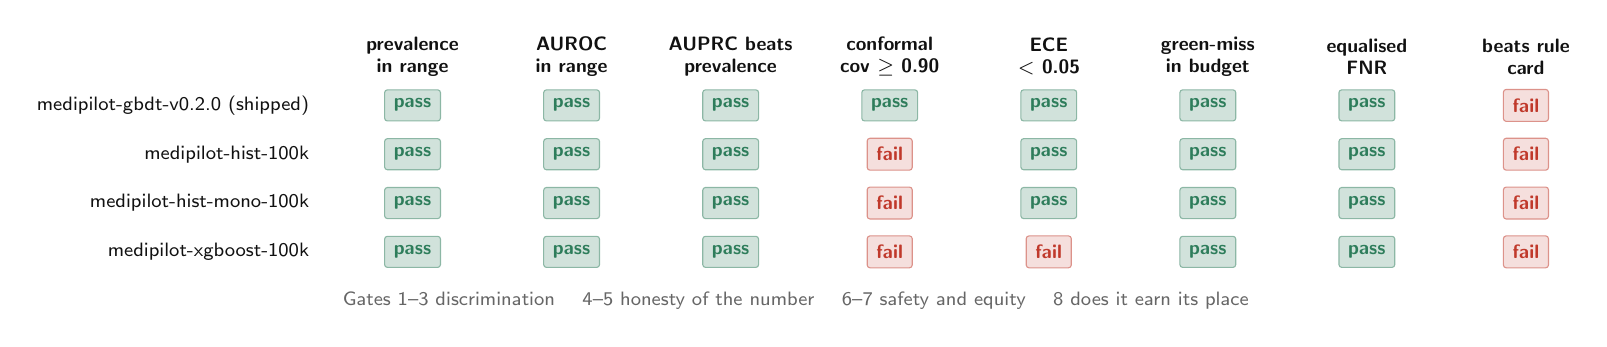
\begin{tikzpicture}[font=\sffamily\scriptsize,
  pass/.style={fill=TriGreen!22,draw=TriGreen!55},
  fail/.style={fill=TriRed!16,draw=TriRed!55}]
\def\cw{2.02}\def\ch{0.62}
% gate headers
\foreach \g/\lbl [count=\i from 0] in {
  1/{prevalence\\in range}, 2/{AUROC\\in range}, 3/{AUPRC beats\\prevalence},
  4/{conformal\\cov $\ge$ 0.90}, 5/{ECE\\$<$ 0.05}, 6/{green-miss\\in budget},
  7/{equalised\\FNR}, 8/{beats rule\\card}} {
  \node[align=center,text=NearBlack,font=\sffamily\scriptsize\bfseries]
    at ({\i*\cw+\cw/2},{0.62}) {\lbl};
}
% rows: 1 = pass, 0 = fail
\foreach \m/\name/\res [count=\r from 0] in {
  0/{medipilot-gbdt-v0.2.0 (shipped)}/{1,1,1,1,1,1,1,0},
  1/{medipilot-hist-100k}/{1,1,1,0,1,1,1,0},
  2/{medipilot-hist-mono-100k}/{1,1,1,0,1,1,1,0},
  3/{medipilot-xgboost-100k}/{1,1,1,0,0,1,1,0}} {
  \node[anchor=east,text=NearBlack] at ({-0.18},{-\r*\ch}) {\name};
  \foreach \v [count=\c from 0] in \res {
    \ifnum\v=1
      \node[pass,minimum width={\cw-0.10cm},minimum height={\ch-0.10cm},
            rounded corners=1pt,text=TriGreen]
        at ({\c*\cw+\cw/2},{-\r*\ch}) {\textbf{pass}};
    \else
      \node[fail,minimum width={\cw-0.10cm},minimum height={\ch-0.10cm},
            rounded corners=1pt,text=TriRed]
        at ({\c*\cw+\cw/2},{-\r*\ch}) {\textbf{fail}};
    \fi
  }
}
\node[anchor=west,text=MedGray,font=\sffamily\scriptsize]
  at ({0},{-3*\ch-0.62}) {Gates 1--3 discrimination \quad 4--5 honesty of the number \quad 6--7 safety and equity \quad 8 does it earn its place};
\end{tikzpicture}}
\caption{The eight go-live gates across the bake-off, on the common held-out split. No artifact is
deployable until all eight pass \emph{on the site's own shadow-mode data}. Two columns carry the
story: gate~4 (conformal coverage) is where the three 100k models fail --- a confidence band that
does not cover at its stated rate is worse than no band --- and gate~8 fails for every candidate,
because none reliably beats the hand-coded rule card at tight operating points. The shipped model
is the only one that clears the honesty gates, which is why it ships.}
\label{fig:gates}
\end{figure*}

\subsection{The safety metric, not accuracy}
Accuracy is meaningless at 10\% prevalence. The metric that governs is under-triage at a fixed
over-triage rate: how many critical patients are left below Yellow when the department can tolerate
a given false-alarm load.

\begin{figure}[t]
\centering
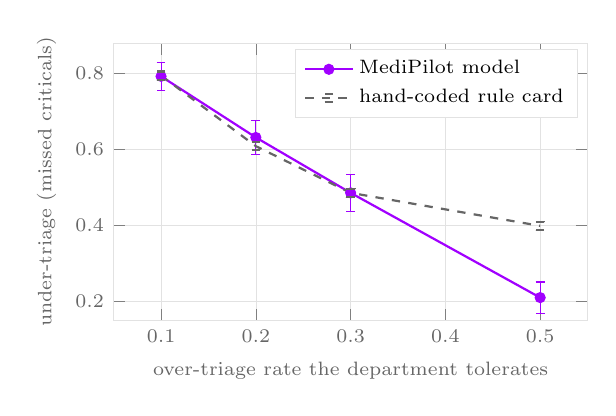
\begin{tikzpicture}
\begin{axis}[
  width=7.6cm, height=5.1cm,
  xlabel={\scriptsize over-triage rate the department tolerates},
  ylabel={\scriptsize under-triage (missed criticals)},
  xlabel style={font=\scriptsize,color=MedGray},
  ylabel style={font=\scriptsize,color=MedGray},
  tick label style={font=\scriptsize,color=MedGray},
  xmin=0.05,xmax=0.55, ymin=0.15, ymax=0.88,
  grid=major, grid style={Border,very thin},
  axis line style={Border},
  legend style={font=\scriptsize,draw=Border,fill=White,at={(0.98,0.98)},anchor=north east},
  legend cell align=left,
]
\addplot[AccPurple,thick,mark=*,mark size=1.6pt,
  error bars/.cd, y dir=both, y explicit]
 coordinates {
  (0.10,0.793) +- (0,0.037)
  (0.20,0.632) +- (0,0.045)
  (0.30,0.486) +- (0,0.048)
  (0.50,0.210) +- (0,0.041)
 };
\addlegendentry{MediPilot model}
\addplot[MedGray,thick,dashed,mark=square,mark size=1.5pt]
 coordinates {(0.10,0.795) (0.20,0.609) (0.30,0.486) (0.50,0.399)};
\addlegendentry{hand-coded rule card}
\end{axis}
\end{tikzpicture}
\caption{Under-triage at four matched over-triage rates, with bootstrap 95\% CIs, on the shipped
model's committed split. The curves are statistically indistinguishable until the department can
tolerate a 50\% over-triage load, where the model halves the misses (0.210 vs 0.399). This single
separation is the honest extent of the learned model's measured advantage on snapshot scoring.}
\label{fig:undertriage}
\end{figure}

\subsection{Calibration, coverage and fairness}
Fairness is defined as \textbf{equalised false-negative rate across strata} with bootstrap CIs ---
never a bare max--min gap, which at these positive counts would be mostly noise.

\begin{figure}[t]
\centering
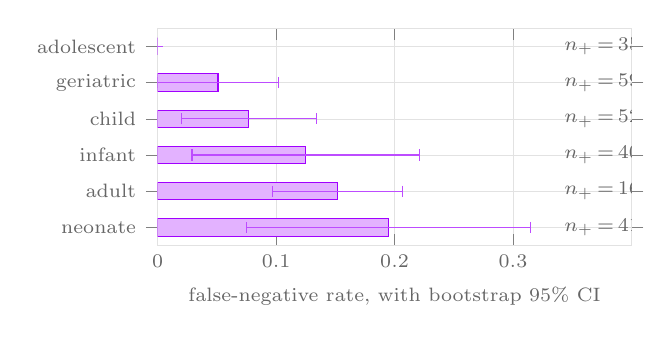
\begin{tikzpicture}
\begin{axis}[
  width=7.6cm, height=5.0cm,
  xbar, xmin=0, xmax=0.40,
  y=0.46cm, bar width=0.22cm,
  symbolic y coords={neonate,adult,infant,child,geriatric,adolescent},
  ytick=data,
  yticklabel style={font=\scriptsize,color=MedGray},
  xlabel={\scriptsize false-negative rate, with bootstrap 95\% CI},
  xlabel style={font=\scriptsize,color=MedGray},
  xtick={0,0.1,0.2,0.3},
  tick label style={font=\scriptsize,color=MedGray},
  grid=major, grid style={Border,very thin},
  axis line style={Border},
]
\addplot[fill=AccPurple!30,draw=AccPurple,
  error bars/.cd, x dir=both, x explicit,
  error bar style={AccPurple!70,thin}]
 coordinates {
  (0.195,neonate)    +- (0.120,0.130)
  (0.152,adult)      +- (0.055,0.058)
  (0.125,infant)     +- (0.096,0.112)
  (0.077,child)      +- (0.057,0.083)
  (0.051,geriatric)  +- (0.051,0.070)
  (0.000,adolescent) +- (0.000,0.000)
 };
\node[font=\scriptsize,color=MedGray,anchor=west] at (axis cs:0.335,neonate)    {$n_{+}$\,=\,41};
\node[font=\scriptsize,color=MedGray,anchor=west] at (axis cs:0.335,adult)      {$n_{+}$\,=\,164};
\node[font=\scriptsize,color=MedGray,anchor=west] at (axis cs:0.335,infant)     {$n_{+}$\,=\,40};
\node[font=\scriptsize,color=MedGray,anchor=west] at (axis cs:0.335,child)      {$n_{+}$\,=\,52};
\node[font=\scriptsize,color=MedGray,anchor=west] at (axis cs:0.335,geriatric)  {$n_{+}$\,=\,59};
\node[font=\scriptsize,color=MedGray,anchor=west] at (axis cs:0.335,adolescent) {$n_{+}$\,=\,35};
\end{axis}
\end{tikzpicture}
\caption{False-negative rate by age stratum for the shipped model, with bootstrap CIs and positive
counts. The spread is 0.195. Neonates are the worst-served stratum on 41 positives --- a real
finding with genuinely wide error bars, and the single clearest argument for the paediatric data
partnership in Phase~2 (\S\ref{sec:roadmap}).}
\label{fig:fairness}
\end{figure}

Calibration is strong and uniform: overall ECE 0.011 with a reliability slope of 0.954 and
intercept $-0.083$, and per-stratum ECE between 0.017 (neonate) and 0.033 (adolescent), reportable
in all six. Conformal coverage is 0.910 overall with a mean set size of 1.08 --- the guarantee is
met while the set stays informative, which is the difficulty with conformal methods in practice.

\subsection{Time to detection --- the number the product is for}
Everything above scores a \emph{snapshot}. The claim this product actually makes is temporal, so
we measured it directly. Every corpus patient carries a 37-step trajectory; we rebuilt the feature
row at each 5-minute step through the same extractor the model was trained on, scored it with the
shipped artifact, and read off two detection times from the same curve --- the first 5-minute tick
that crosses the threshold, and the first \emph{scheduled} physical re-measurement at or after it
on the band's own cadence (\pth{eval/time\_to\_detection.py}).

\begin{figure}[t]
\centering
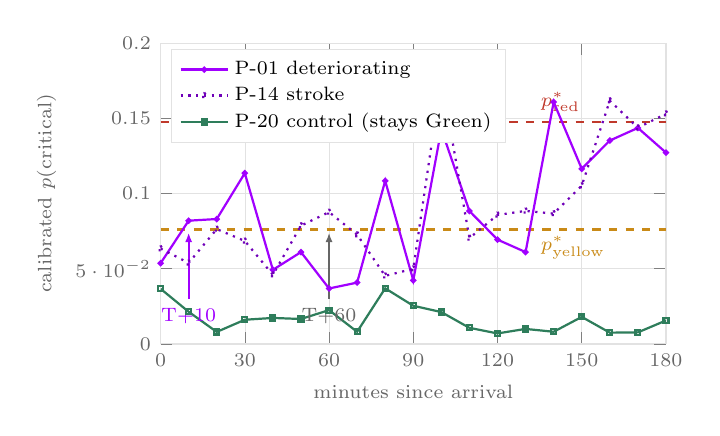
\begin{tikzpicture}
\begin{axis}[
  width=8.0cm, height=5.4cm,
  xlabel={\scriptsize minutes since arrival},
  ylabel={\scriptsize calibrated $p$(critical)},
  xlabel style={font=\scriptsize,color=MedGray},
  ylabel style={font=\scriptsize,color=MedGray},
  tick label style={font=\scriptsize,color=MedGray},
  xmin=0,xmax=180, ymin=0, ymax=0.20,
  xtick={0,30,60,90,120,150,180},
  ytick={0,0.05,0.10,0.15,0.20},
  grid=major, grid style={Border,very thin},
  axis line style={Border},
  legend style={font=\scriptsize,draw=Border,fill=White,
                at={(0.02,0.98)},anchor=north west,row sep=-1pt},
  legend cell align=left,
]
% threshold lines
\addplot[TriRed,dashed,thick,forget plot] coordinates {(0,0.1473) (180,0.1473)};
\addplot[TriAmber,dashed,thick,forget plot] coordinates {(0,0.0760) (180,0.0760)};
\node[font=\scriptsize,color=TriRed,anchor=west]   at (axis cs:132,0.1610) {$p^{*}_{\text{red}}$};
\node[font=\scriptsize,color=TriAmber,anchor=west] at (axis cs:132,0.0640) {$p^{*}_{\text{yellow}}$};

\addplot[AccPurple,thick,mark=*,mark size=0.7pt] coordinates {
(0,0.0536) (10,0.0819) (20,0.0830) (30,0.1135) (40,0.0492) (50,0.0610)
(60,0.0368) (70,0.0407) (80,0.1084) (90,0.0422) (100,0.1427) (110,0.0883)
(120,0.0693) (130,0.0610) (140,0.1608) (150,0.1164) (160,0.1352)
(170,0.1436) (180,0.1272)};
\addlegendentry{P-01 deteriorating}

\addplot[SecPurple,thick,dotted,mark=triangle,mark size=1.1pt] coordinates {
(0,0.0633) (10,0.0538) (20,0.0763) (30,0.0684) (40,0.0459) (50,0.0786)
(60,0.0876) (70,0.0726) (80,0.0452) (90,0.0499) (100,0.1769) (110,0.0703)
(120,0.0857) (130,0.0884) (140,0.0866) (150,0.1052) (160,0.1617)
(170,0.1437) (180,0.1530)};
\addlegendentry{P-14 stroke}

\addplot[TriGreen,thick,mark=square,mark size=0.9pt] coordinates {
(0,0.0366) (10,0.0213) (20,0.0079) (30,0.0160) (40,0.0172) (50,0.0165)
(60,0.0224) (70,0.0080) (80,0.0369) (90,0.0253) (100,0.0211) (110,0.0106)
(120,0.0069) (130,0.0099) (140,0.0080) (150,0.0179) (160,0.0074)
(170,0.0076) (180,0.0155)};
\addlegendentry{P-20 control (stays Green)}

% detection markers for P-01
\draw[AccPurple,thick,-{Latex[length=1.2mm]}] (axis cs:10,0.030) -- (axis cs:10,0.074);
\node[font=\scriptsize,color=AccPurple,anchor=north] at (axis cs:10,0.030) {T+10};
\draw[MedGray,thick,-{Latex[length=1.2mm]}] (axis cs:60,0.030) -- (axis cs:60,0.074);
\node[font=\scriptsize,color=MedGray,anchor=north] at (axis cs:60,0.030) {T+60};
\end{axis}
\end{tikzpicture}
\caption{Calibrated risk over the full 180-minute wait, scored every five minutes with the shipped
artifact. \pid{P-01} crosses the Yellow threshold at \textbf{T+10}; the next \emph{scheduled}
physical re-measurement on the Green cadence would not arrive until \textbf{T+60} --- a 50-minute
head start. \pid{P-20} is the control and never approaches the threshold, which is what makes the
comparison meaningful. The curves are deliberately not smoothed: real vitals are noisy, and the
escalation-only invariant is what makes that noise safe --- a spurious high reading can only ratchet
priority \emph{up}, and a spurious low one cannot pull it down.}
\label{fig:ptcurve}
\end{figure}

\begin{figure}[t]
\centering
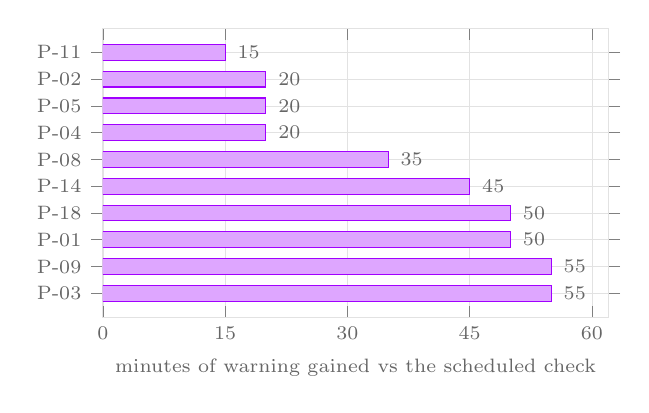
\begin{tikzpicture}
\begin{axis}[
  width=8.0cm, height=5.0cm,
  xbar, xmin=0, xmax=62,
  y=0.34cm, bar width=0.20cm,
  symbolic y coords={P-03,P-09,P-01,P-18,P-14,P-08,P-04,P-05,P-02,P-11},
  ytick=data,
  yticklabel style={font=\scriptsize,color=MedGray},
  xlabel={\scriptsize minutes of warning gained vs the scheduled check},
  xlabel style={font=\scriptsize,color=MedGray},
  tick label style={font=\scriptsize,color=MedGray},
  xtick={0,15,30,45,60},
  grid=major, grid style={Border,very thin},
  axis line style={Border},
  nodes near coords, point meta=explicit symbolic,
  every node near coord/.append style={font=\scriptsize,color=MedGray,
                                       anchor=west,xshift=1pt},
]
\addplot[fill=AccPurple!35,draw=AccPurple] coordinates {
 (55,P-03) [55] (55,P-09) [55] (50,P-01) [50] (50,P-18) [50] (45,P-14) [45]
 (35,P-08) [35] (20,P-04) [20] (20,P-05) [20] (20,P-02) [20] (15,P-11) [15]};
\end{axis}
\end{tikzpicture}
\caption{Head start per patient at the Yellow threshold: how many minutes earlier continuous
five-minute re-scoring reaches the threshold than the next scheduled re-measurement would.
Across the 16 of 20 corpus patients who cross at all, the mean gain is \textbf{21.6 minutes} and
the median \textbf{17.5}. Ten patients are shown; the remaining six cross at T=0 and gain nothing,
because they were already deteriorating on arrival --- those are cases the initial assessment
catches, and the system is not claiming credit for them.}
\label{fig:headstart}
\end{figure}

\textbf{Sixteen of twenty patients cross the Yellow threshold during the wait.} Across those,
continuous re-scoring gets there a mean of \textbf{21.6 minutes} earlier than the scheduled check,
median 17.5, maximum 55. Two patients would have lost a full cadence. At the Red threshold, which
eight patients reach, the mean gain is 6.9 minutes --- smaller, and honestly so: Red crossings tend
to be dramatic enough that the shorter Yellow-band cadence catches them soon anyway. \emph{The
value is concentrated in the Yellow queue, which is exactly where the brief says people die.}


\subsection{8/8 or 7/8 --- and why the difference is the point}
No artifact is deployable until all eight gates pass on the site's own shadow-mode data. The
shipped artifact clears \textbf{8/8} on its own committed split ($n{=}4{,}001$) and \textbf{7/8}
on the fresh common split ($n{=}20{,}000$). Exactly one gate moves, and it is gate~8. On the
smaller split the model wins at otr~0.50 and loses nowhere, because the intervals are too wide to
separate; on the split five times larger they tighten until a loss at otr~0.20 becomes significant,
and the gate flips. \textbf{We report the stricter result.} The full ledger, both splits side by
side, is Table~\ref{tab:gateledger}.

\subsection{LLM structurer bake-off --- ten candidates}
The language model is confined to perception, and this evaluation is how that confinement is
\emph{measured} rather than asserted. Ten candidates were scored on a deliberately messy case set
covering adversarial, ambiguous, negation, Hinglish, prompt-injection, obstetric, paediatric,
stroke and reliability slices.

\begin{center}\footnotesize\sffamily
\begin{tabular}{@{}p{1.95cm}p{0.78cm}p{0.86cm}p{1.05cm}p{0.98cm}@{}}
\toprule
\rowcolor{AccPurple!10}
\textbf{Candidate} & \textbf{F1} & \textbf{RF}\newline\textbf{miss} & \textbf{Schema}\newline\textbf{fail} & \textbf{Lat. (s)}\\
\midrule
\rowcolor{AccPurple!7}
gpt-oss-120b \emph{(chosen)} & \textbf{0.962} & \textbf{0} & 0 & 7.59\\
\rowcolor{AccPurple!7}
gpt-oss-20b \emph{(chosen, fast)} & 0.816 & 4 & 4 & 8.89\\
Qwen2.5-7B (local) & 0.653 & 7 & 0 & 5.46\\
Qwen2.5-3B (local) & 0.650 & 8 & 0 & 6.42\\
Phi-4-mini (local) & 0.608 & 3 & 0 & 5.65\\
Qwen2.5-1.5B (local) & 0.528 & 11 & 0 & 4.04\\
\emph{Rule baseline (no LLM)} & 0.510 & 12 & 0 & \textbf{0.00}\\
llama-3.3-70b & 0.325 & 18 & \textbf{40} & 0.15\\
llama-3.1-8b & 0.325 & 18 & 40 & 0.10\\
kimi-k2-instruct & 0.325 & 18 & 40 & 0.08\\
\bottomrule
\end{tabular}
\end{center}

\vspace{3pt}
Two results matter commercially. First, \textbf{the three largest instruction-tuned models are the
worst performers here} --- 40 schema failures each, meaning they would not emit the constrained
form at all. Capability and constrained-decoding compliance are different properties, and buying
the biggest model would have been the wrong decision. Second, \textbf{the rule baseline misses 12
red flags and the chosen model misses zero}, which is exactly why the deterministic structurer is
the floor and not the default --- and why losing the network degrades the system rather than
stopping it.

\begin{figure}[t]
\centering
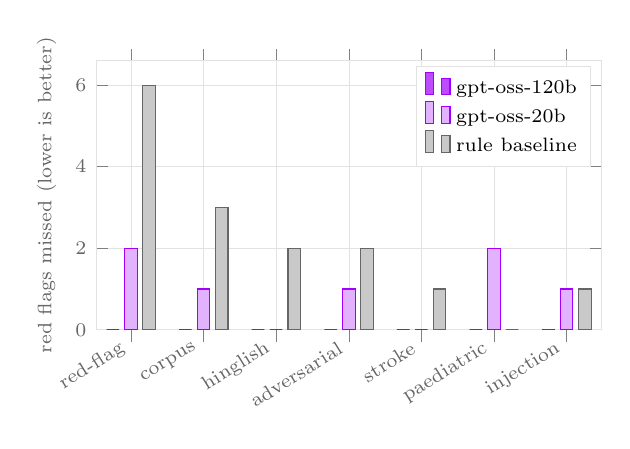
\begin{tikzpicture}
\begin{axis}[
  ybar, width=8.0cm, height=5.0cm,
  bar width=0.16cm,
  enlarge x limits=0.08,
  ymin=0, ymax=6.6,
  ylabel={\scriptsize red flags missed (lower is better)},
  ylabel style={font=\scriptsize,color=MedGray},
  symbolic x coords={red-flag,corpus,hinglish,adversarial,stroke,paediatric,injection},
  xtick=data,
  x tick label style={font=\scriptsize,color=MedGray,rotate=32,anchor=east},
  tick label style={font=\scriptsize,color=MedGray},
  grid=major, grid style={Border,very thin},
  axis line style={Border},
  legend style={font=\scriptsize,draw=Border,fill=White,
                at={(0.98,0.98)},anchor=north east,row sep=-1pt},
  legend cell align=left,
]
\addplot[fill=AccPurple!70,draw=AccPurple] coordinates {
 (red-flag,0) (corpus,0) (hinglish,0) (adversarial,0) (stroke,0) (paediatric,0) (injection,0)};
\addlegendentry{gpt-oss-120b}
\addplot[fill=AccPurple!30,draw=AccPurple] coordinates {
 (red-flag,2) (corpus,1) (hinglish,0) (adversarial,1) (stroke,0) (paediatric,2) (injection,1)};
\addlegendentry{gpt-oss-20b}
\addplot[fill=MedGray!35,draw=MedGray] coordinates {
 (red-flag,6) (corpus,3) (hinglish,2) (adversarial,2) (stroke,1) (paediatric,0) (injection,1)};
\addlegendentry{rule baseline}
\end{axis}
\end{tikzpicture}
\caption{Red flags missed per evaluation slice --- the only structurer metric with a body count.
\cm{gpt-oss-120b} misses none anywhere, including the code-mixed Hinglish and prompt-injection
slices. The rule baseline misses six on the red-flag slice alone and is the only candidate that
fails on stroke. Note the \emph{paediatric} column: \cm{gpt-oss-20b} misses two where the rule
baseline misses none, which is precisely why the 20b model is confined to option matching and
classification while the 120b does observation extraction.}
\label{fig:slices}
\end{figure}

\subsection{ASR bake-off --- twelve backends}
Transcription was selected on measured word error rate, not on a datasheet.
\cm{whisper-large-v3-turbo} through the hosted path and \cm{whisper-local:turbo} both reach WER
0.000 on the reference utterances, with hosted latency 0.30\,s against 1.21\,s locally and a
4.94\,GB VRAM footprint for the local path. Nine other backends --- including
\cm{faster-whisper:large-v3} at both \cm{int8\_float16} and \cm{float16}, which score WER 0.583 ---
were rejected on measurement. \textbf{Zero silence hallucinations were recorded across every
backend}, which is the result the pre-flight RMS silence gate exists to guarantee.

\begin{figure}[t]
\centering
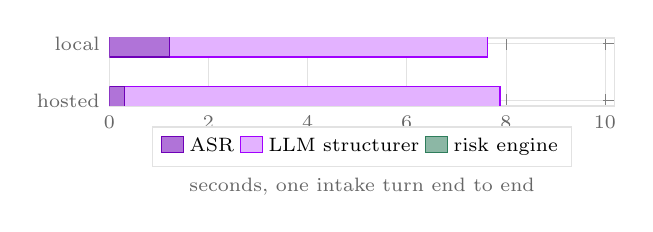
\begin{tikzpicture}
\begin{axis}[
  xbar stacked, width=8.0cm, height=3.5cm,
  xmin=0, xmax=10.2,
  y=0.72cm, bar width=0.34cm,
  symbolic y coords={hosted,local},
  ytick=data,
  yticklabel style={font=\scriptsize,color=MedGray},
  xlabel={\scriptsize seconds, one intake turn end to end},
  xlabel style={font=\scriptsize,color=MedGray,yshift=-11pt},
  tick label style={font=\scriptsize,color=MedGray},
  grid=major, grid style={Border,very thin},
  axis line style={Border},
  legend style={font=\scriptsize,draw=Border,fill=White,
                at={(0.5,-0.30)},anchor=north,legend columns=3,row sep=-1pt},
  legend cell align=left,
]
\addplot[fill=SecPurple!55,draw=SecPurple] coordinates {(0.298,hosted) (1.206,local)};
\addlegendentry{ASR}
\addplot[fill=AccPurple!30,draw=AccPurple] coordinates {(7.586,hosted) (6.421,local)};
\addlegendentry{LLM structurer}
\addplot[fill=TriGreen!55,draw=TriGreen] coordinates {(0.003,hosted) (0.003,local)};
\addlegendentry{risk engine}
\end{axis}
\end{tikzpicture}
\caption{Where the time actually goes in one intake turn. The \textbf{risk engine is 3\,ms} --- a
measured p50 over 300 calls, with p95 4.3\,ms and p99 8.0\,ms --- and is invisible on this scale.
Effectively all latency is perception, and the structurer dominates it. This is an architecturally
useful result: the expensive component is the one that may only \emph{report}, so it can be
degraded, cached or dropped to the offline tier without touching the component that decides.}
\label{fig:latency}
\end{figure}

\begin{figure}[t]
\centering
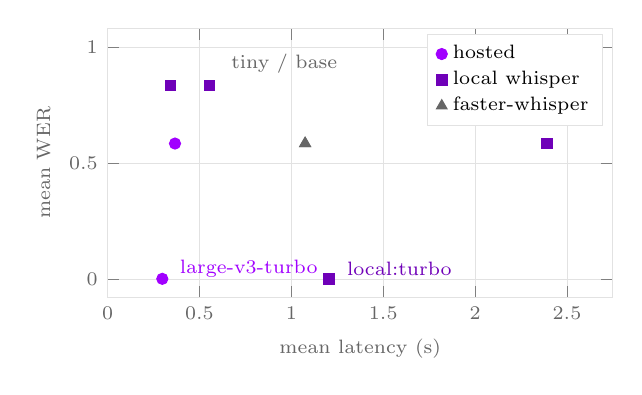
\begin{tikzpicture}
\begin{axis}[
  width=8.0cm, height=5.0cm,
  xlabel={\scriptsize mean latency (s)}, ylabel={\scriptsize mean WER},
  xlabel style={font=\scriptsize,color=MedGray},
  ylabel style={font=\scriptsize,color=MedGray},
  tick label style={font=\scriptsize,color=MedGray},
  xmin=0, xmax=2.75, ymin=-0.08, ymax=1.08,
  grid=major, grid style={Border,very thin},
  axis line style={Border},
  legend style={font=\scriptsize,draw=Border,fill=White,
                at={(0.98,0.98)},anchor=north east,row sep=-1pt},
  legend cell align=left,
]
\addplot[only marks,mark=*,mark size=2.0pt,AccPurple] coordinates {
 (0.298,0.000) (0.367,0.583)};
\addlegendentry{hosted}
\addplot[only marks,mark=square*,mark size=1.9pt,SecPurple] coordinates {
 (1.206,0.000) (2.392,0.583) (2.309,0.750) (0.554,0.833) (0.343,0.833)};
\addlegendentry{local whisper}
\addplot[only marks,mark=triangle*,mark size=2.2pt,MedGray] coordinates {
 (1.076,0.583) (1.074,0.583) (0.562,3.750)};
\addlegendentry{faster-whisper}
\node[font=\scriptsize,color=AccPurple,anchor=west]  at (axis cs:0.34,0.045) {large-v3-turbo};
\node[font=\scriptsize,color=SecPurple,anchor=west]  at (axis cs:1.25,0.045) {local:turbo};
\node[font=\scriptsize,color=MedGray,anchor=south west] at (axis cs:0.62,0.845) {tiny / base};
\end{axis}
\end{tikzpicture}
\caption{ASR selection on measurement rather than on a datasheet. Two backends reach WER 0.000;
the hosted turbo path is 4$\times$ faster than the local one, and the local path costs 4.94\,GB of
VRAM. Everything at WER 0.583 and above was rejected --- including both \cm{faster-whisper:large-v3}
quantisations, which a specification sheet would have ranked highly. \cm{faster-whisper:small/int8}
is off-scale at WER 3.750. \textbf{Caveat: only two reference utterances}, so this separates the
field but does not settle it (\S\ref{sec:data}).}
\label{fig:asr}
\end{figure}

\subsection{The invariant suite}
282 tests run on every change, of which 278 pass; the four failures are a packaging artefact and a
stale assertion, both documented in the implementation README. The suite is not a unit-test
formality --- it is where the clinical constraints are enforced: 15 invariant tests, 10 on age
stratification, 10 replaying the corpus acceptance cases, 8 on surge control, 7 on the band engine,
6 on the audit log and 6 on reliability weighting.

% ======================= 7. USERS =======================
\section{Target Users and Adoption}
\label{sec:users}

\begin{figure*}[t]
  \centering
  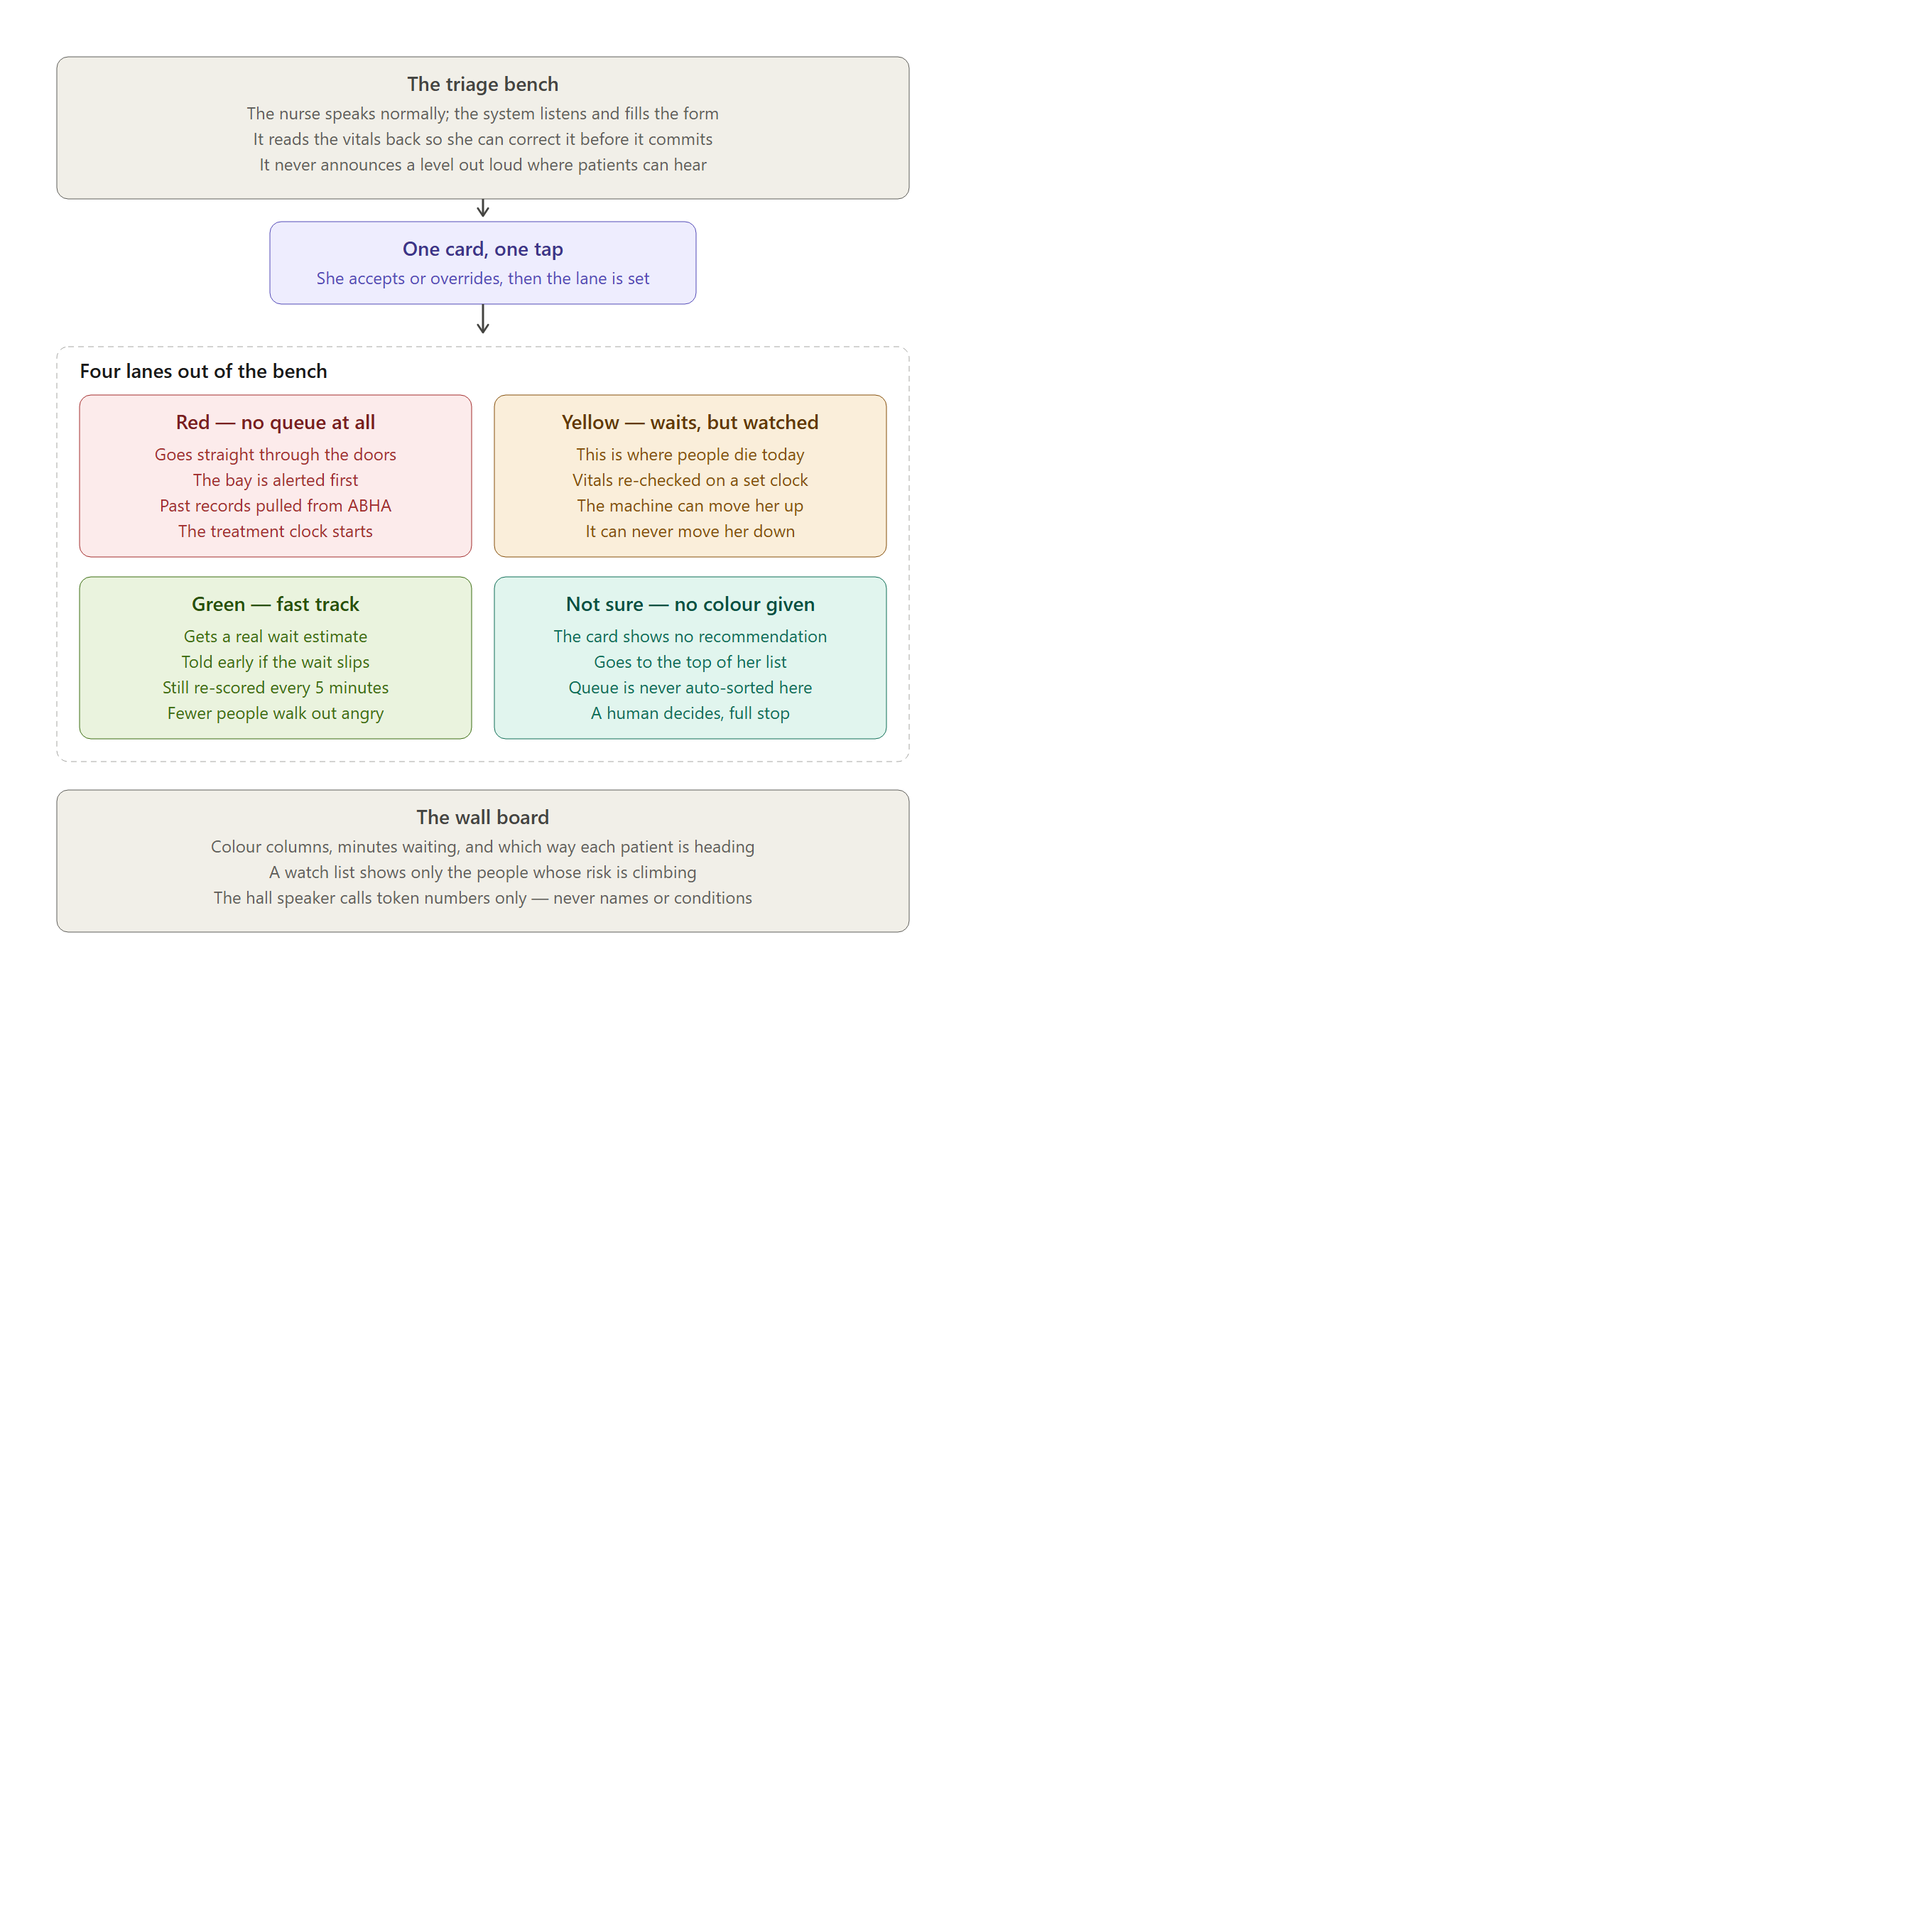
\includegraphics[trim=59 1371 1419 59,clip,width=0.70\textwidth]{../diagrams/03-in-the-room-lanes-and-voice.png}
  \caption{What each user actually experiences. The abstention lane is a first-class outcome rather
  than an error state: no colour is offered, the queue is never auto-sorted, and a human decides.}
  \label{fig:lanes}
\end{figure*}

\subsection{Five users, three of whom are not clinicians}
\begin{center}\footnotesize\sffamily
\begin{tabular}{@{}p{1.85cm}p{5.95cm}@{}}
\toprule
\rowcolor{AccPurple!10}
\textbf{User} & \textbf{What they get, and what they can do}\\
\midrule
Triage nurse & The primary user. One card, two supporting factors, one opposing factor, a confidence band. Accept or override in one touch. Gains a continuous monitoring layer she cannot physically provide\\
\addlinespace[2pt]
Patient & Speaks Hindi or English to a kiosk, or taps. Never told a colour out loud. Gets a real wait estimate and is told early if it slips\\
\addlinespace[2pt]
Family / attendant & Can perform and close a \emph{Green} recheck only; doing so raises a flag for staff. Recognises that families already participate in care in Indian EDs, without granting clinical authority\\
\addlinespace[2pt]
Counter / office staff & Registration and token issue. Sees queue position, never risk scores\\
\addlinespace[2pt]
Clinical governance & The audit ledger, override patterns, drift alarms, and sign-off on every YAML change\\
\bottomrule
\end{tabular}
\end{center}

\subsection{Adoption --- designed against the failure modes of clinical AI}
Fatigued staff work around tools that add work or insult their judgement. Six choices follow
directly:

\begin{itemize}
  \item \textbf{Zero workflow change to start.} The wedge module never assigns an initial acuity;
        it watches a queue the nurse already ordered. Nothing is taken away.
  \item \textbf{The opposing factor.} Every card names the strongest evidence \emph{against} its
        own recommendation. This forces engagement with reasoning rather than with a number, and it
        is the standard defence against automation bias.
  \item \textbf{Override is one touch and is never punished.} It is a first-class route in the API,
        not an escape hatch.
  \item \textbf{Abstention is visible.} A system that says "I don't know" on the $\sim$8\% it
        genuinely cannot judge earns trust on the remainder.
  \item \textbf{No virtual-nurse persona.} No avatar, no manufactured clinical authority.
  \item \textbf{Shadow mode first.} Staff see the system's judgement compared against their own for
        weeks before it is allowed to surface anything.
\end{itemize}

% ======================= 8. REGULATORY =======================
\section{Data Protection and Regulatory Position}
\label{sec:reg}

\subsection{Stated jurisdiction: India}
\textbf{DPDP Act 2023}, the ABDM consent framework, ICMR's 2023 AI ethics guidance, and the CDSCO
draft guidance on AI/ML medical device software including algorithm change protocols.

\begin{tcolorbox}[mpbox]
\textbf{The gap we name rather than paper over.} ABDM consent for care delivery does \emph{not} by
itself satisfy DPDP Act 2023 for using the same data as model input. These are different purposes
and require separate, revocable consent. Any vendor claiming ABDM integration equals DPDP
compliance for training is wrong, and this is the single largest regulatory item on our roadmap.
\end{tcolorbox}

\subsection{How the data is actually protected}
\textbf{On-premise by default.} With no API credential configured the system runs entirely inside
the hospital: local ASR, offline phrase matching, the deterministic structurer, and no outbound
request on any path. Privacy is a deployment mode, not a policy document.

\textbf{Only model updates travel.} Cross-site learning is federated with secure aggregation ---
weights move, patient data does not. Per-site calibration stays local.

\textbf{The audit ledger.} Every autonomous decision and every override appends a record with 17
substantive fields plus two hash-chain fields. It is append-only and SHA-256 hash-chained, so a
retroactive edit is mathematically detectable. Consent withdrawal is recorded as a \emph{new event},
never as a deletion, which is what preserves the integrity of the chain while honouring the
withdrawal.

\textbf{What a clinician override legally records.} Named clinician and role, system band and
clinician band, direction, reason code and free text, the calibrated score and confidence at that
moment, the factors as displayed on the card, an inputs hash, model and calibration versions, and
the consent state. \cm{outcome\_ref} is back-filled when known --- and that back-fill is the
training signal.

% ======================= 9. BUSINESS =======================
\section{Business Case and Impact}
\label{sec:business}

\subsection{Unit economics}
\begin{tcolorbox}[mpwarn]
The figures below are an \textbf{illustrative model under stated assumptions}, not measured
revenue. No pilot has been run and no price has been agreed.
\end{tcolorbox}

Assume the brief's range of 100--500 visits per day. The architecture is deliberately cheap because
the required path has no GPU and no per-token cost: the risk model is gradient-boosted trees at
millisecond latency on commodity CPU, and the language model is optional. The white paper's design
target is \textbf{under Rs.\,5 per encounter} at the edge tier.

\begin{center}\footnotesize\sffamily
\begin{tabular}{@{}p{2.35cm}p{1.35cm}p{1.85cm}p{1.4cm}@{}}
\toprule
\rowcolor{AccPurple!10}
\textbf{Site} & \textbf{Visits/day} & \textbf{Enc./yr} & \textbf{At Rs.\,5}\\
\midrule
District hospital & 100 & 36{,}500 & Rs.\,1.8 L/yr\\
Mid-size urban ED & 250 & 91{,}250 & Rs.\,4.6 L/yr\\
Tertiary trauma centre & 500 & 182{,}500 & Rs.\,9.1 L/yr\\
\bottomrule
\end{tabular}
\end{center}

\subsection{Where the value lands}
The economic case does not rest on staff replacement --- headcount is unchanged. It rests on four
effects, ordered by how directly they are measurable:

\begin{enumerate}
  \item \textbf{Deterioration caught during the wait.} The single event the system exists to
        prevent. Each avoided in-queue deterioration avoids an ICU escalation.
  \item \textbf{Fewer left-without-being-seen.} Green patients receive a real wait estimate and are
        told when it slips. LWBS is already tracked by most EDs, so this is measurable from day one
        without new instrumentation.
  \item \textbf{Documented defensibility.} A hash-chained audit trail of every recommendation and
        every override is a liability-management asset independent of clinical outcome.
  \item \textbf{Compounding calibration.} Each site improves the model for every other site through
        federated rounds --- an advantage structurally unavailable to a single-site or late entrant.
\end{enumerate}

\subsection{Why this is defensible}
A well-funded competitor can rebuild the technical stack in a year. It cannot rebuild years of
site-specific calibration and federated override history across dozens of Indian EDs. The moat is
the data relationship, not the model.

% ======================= 10. SCALE =======================
\section{Scalability Across Hospitals}
\label{sec:scale}

\begin{figure*}[t]
  \centering
  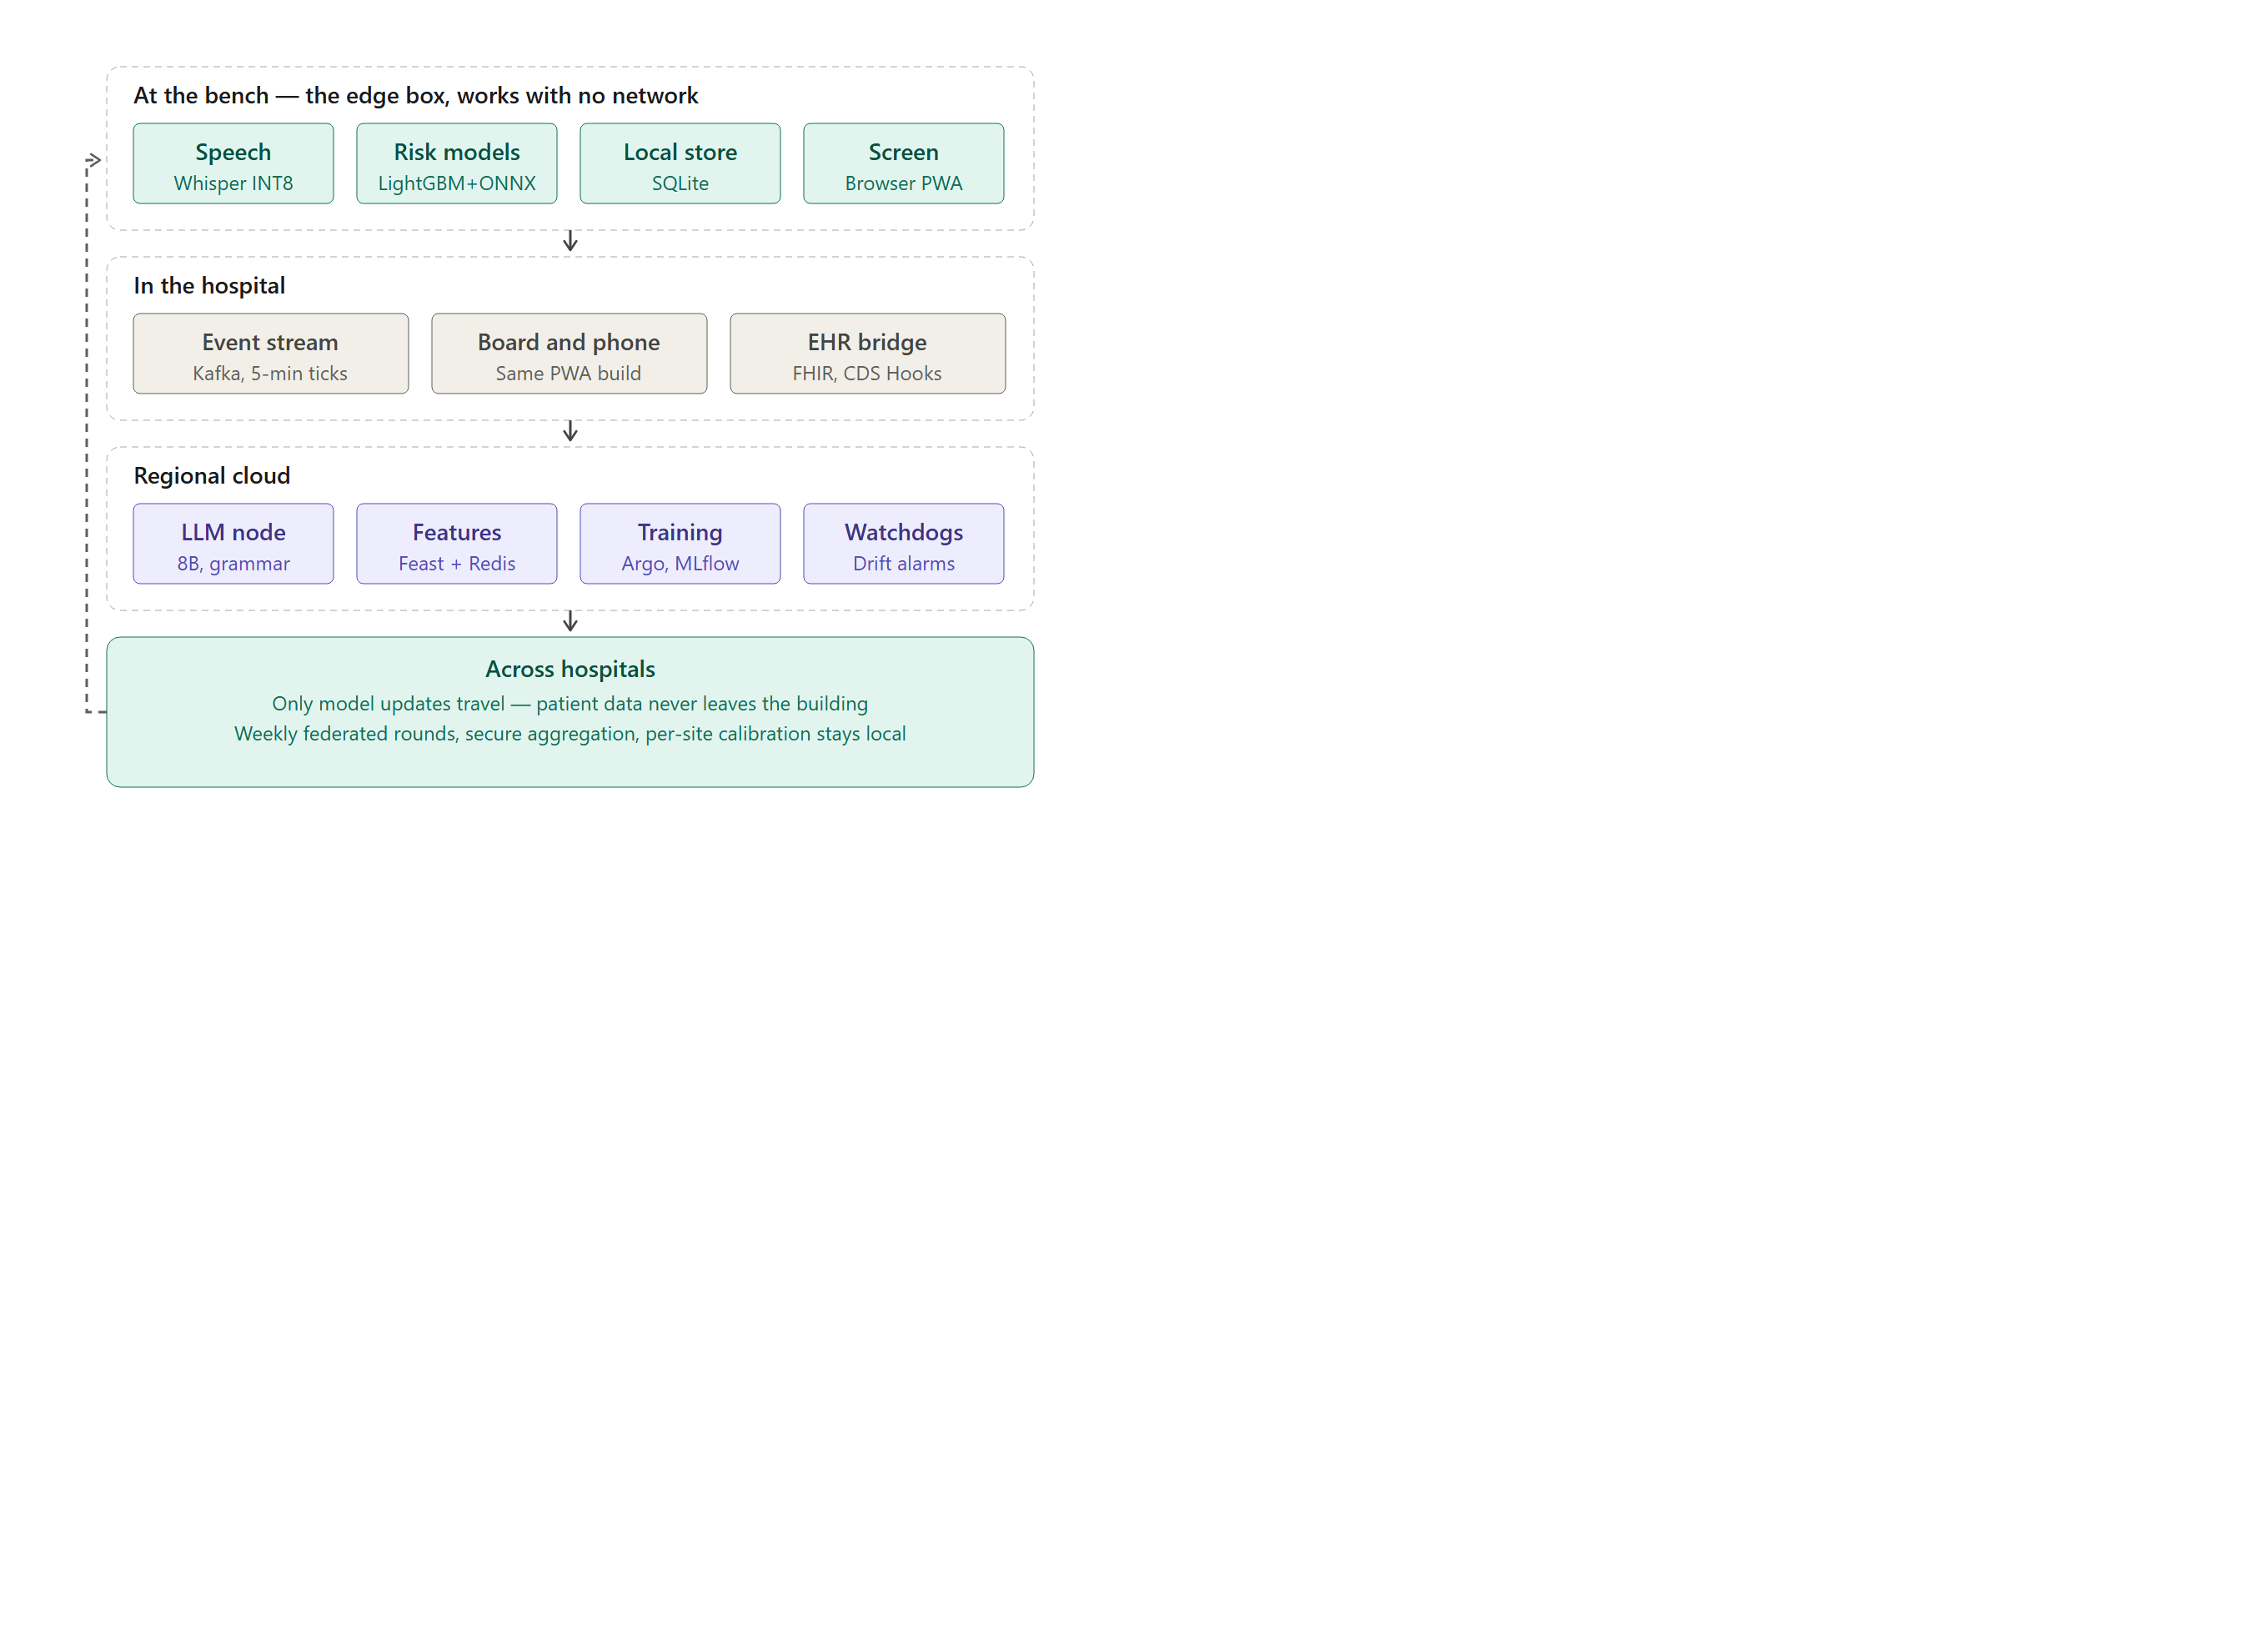
\includegraphics[trim=92 1013 1469 69,clip,width=0.80\textwidth]{../diagrams/04-tech-stack-three-tiers.png}
  \caption{Three deployment tiers. A hospital adopts only the tiers it can support: the bench box
  alone is a complete product. The bottom row is the invariant --- only model updates travel between
  sites, and per-site calibration stays local.}
  \label{fig:tiers}
\end{figure*}

The brief asks how one assistant flexes across hospitals of very different size, specialty mix and
technical maturity. The answer is that \textbf{the tiers are independently adoptable}
(Fig.~\ref{fig:tiers}).

\begin{center}\footnotesize\sffamily
\begin{tabular}{@{}p{1.85cm}p{2.15cm}p{3.4cm}@{}}
\toprule
\rowcolor{AccPurple!10}
\textbf{Maturity} & \textbf{Deploys} & \textbf{What they get}\\
\midrule
No IT department & Bench box only & Offline edge inference, SQLite, browser PWA. Works with the network cut\\
\addlinespace[2pt]
Has a network & + hospital tier & Board and phone on the same build, 5-minute event ticks\\
\addlinespace[2pt]
Has an EHR & + FHIR bridge & The card appears inside the existing workflow via CDS Hooks\\
\addlinespace[2pt]
Multi-site group & + regional cloud & Federated rounds, drift watchdogs, self-hosted structurer\\
\bottomrule
\end{tabular}
\end{center}

\vspace{3pt}
\textbf{The honest engineering constraint.} Today both backend applications hold state in process
--- the orchestrator bootstraps a \cm{World} in its lifespan hook and runs a tick loop. Horizontal
replication therefore requires externalising that state to Postgres and Redis \emph{first};
attempting workers before that produces a system that looks scaled and silently disagrees with
itself. This is the first engineering item in Phase~2, not an afterthought.

% ======================= 11. ROADMAP =======================
\section{Phased Roadmap}
\label{sec:roadmap}

\begin{center}
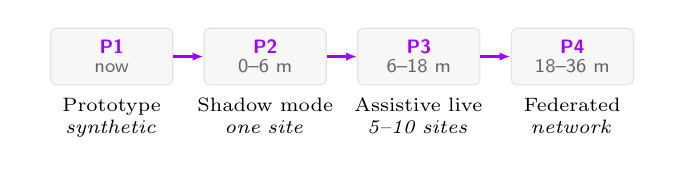
\begin{tikzpicture}[font=\sffamily\scriptsize]
\definecolor{PhA}{HTML}{A100FF}
\foreach \i/\lbl/\sub in {0/{P1}/{now}, 1/{P2}/{0--6 m}, 2/{P3}/{6--18 m}, 3/{P4}/{18--36 m}} {
  \node[draw=Border,fill=CardBg,rounded corners=2pt,minimum width=1.55cm,minimum height=0.72cm,
        align=center] (n\i) at ({\i*1.95},0) {\textbf{\color{AccPurple}\lbl}\\[-1pt]{\color{MedGray}\sub}};
}
\foreach \i in {0,1,2} {
  \draw[-{Latex[length=1.4mm]},AccPurple,thick] (n\i.east) -- (n\the\numexpr\i+1\relax.west);
}
\node[below=1pt of n0,align=center,text width=1.9cm,font=\scriptsize] {Prototype\\ \emph{synthetic}};
\node[below=1pt of n1,align=center,text width=1.9cm,font=\scriptsize] {Shadow mode\\ \emph{one site}};
\node[below=1pt of n2,align=center,text width=1.9cm,font=\scriptsize] {Assistive live\\ \emph{5--10 sites}};
\node[below=1pt of n3,align=center,text width=1.9cm,font=\scriptsize] {Federated\\ \emph{network}};
\end{tikzpicture}
\end{center}

\vspace{2pt}
Each phase has an exit gate that is a measurement, not a date.

{\footnotesize\sffamily
\tablefirsthead{\toprule \rowcolor{AccPurple!10}
  \textbf{Phase} & \textbf{Work} & \textbf{Exit gate}\\ \midrule}
\tablehead{\rowcolor{AccPurple!10}
  \textbf{Phase} & \textbf{Work} & \textbf{Exit gate \itshape(cont.)}\\ \midrule}
\tabletail{}
\tablelasttail{\bottomrule}
\setlength{\tabcolsep}{4pt}
\begin{supertabular}{@{}p{0.95cm}p{2.85cm}p{3.8cm}@{}}
\textbf{P1} & Working prototype on synthetic data. \emph{Complete.} 7 surfaces, 20-patient corpus, 4-model bake-off, 282-test suite &
Every mandated case demonstrable end to end --- \emph{met}\\
\addlinespace[3pt]
\textbf{P2} & Externalise state (Postgres + Redis). Partner site, DPDP/ABDM consent instrument, ethics approval. Shadow mode: model scores silently, nothing surfaced. Paediatric data partnership &
8/8 go-live gates on the \emph{site's own} outcome data; neonate FNR CI narrowed below the adult point estimate\\
\addlinespace[3pt]
\textbf{P3} & Assistive deployment: recommendations surfaced, nurse decides. FHIR/CDS Hooks bridge. ONNX edge box. CDSCO SaMD submission with a predetermined change control plan &
Stepped-wedge cluster randomisation showing reduced in-queue deterioration --- \emph{not} a pre/post comparison\\
\addlinespace[3pt]
\textbf{P4} & Federated rounds with secure aggregation across the network. Drift watchdogs per site. Self-hosted structurer &
Cross-site model improvement demonstrated with zero patient-data egress\\
\end{supertabular}\par}

% ======================= 12. RISKS =======================
\section{Key Risks and Mitigations}
\label{sec:risk}

{\footnotesize\sffamily
\tablefirsthead{\toprule \rowcolor{AccPurple!10}
  \textbf{Risk} & \textbf{Mitigation --- and where it is enforced}\\ \midrule}
\tablehead{\rowcolor{AccPurple!10}
  \textbf{Risk} & \textbf{Mitigation \itshape(cont.)}\\ \midrule}
\tabletail{}
\tablelasttail{\bottomrule}
\begin{supertabular}{@{}p{1.95cm}p{5.85cm}@{}}
Synthetic-to-real gap &
The largest risk in this proposal. No absolute metric transfers. Mitigated only by shadow mode
re-fitting calibration on site data before anything surfaces; the go-live gates are evaluated on
the site's data, never ours\\
\addlinespace[2pt]
Model no better than rules &
\emph{Measured, not hypothetical} (\S\ref{sec:eval}). Mitigated architecturally: the rule card is
the floor, so a model that adds nothing subtracts nothing. The model's distinct value is temporal,
and that is what P3 must demonstrate\\
\addlinespace[2pt]
Neonatal under-triage &
Worst stratum at FNR 0.195. Mitigated by the paediatric data partnership gate in P2 and by
per-stratum thresholds; until then neonates carry the most conservative cut\\
\addlinespace[2pt]
Label leakage &
The failure that broke the Epic Sepsis Model. Mitigated mechanically: leakage classes in the
feature registry, fail-closed on unregistered fields, and a CI canary test\\
\addlinespace[2pt]
Automation bias &
Nurses defer to the screen. Mitigated by the mandatory opposing factor, visible abstention and
override telemetry under clinical governance\\
\addlinespace[2pt]
LLM emits a judgement &
Structurally impossible rather than discouraged: no production rule for acuity exists in the output
grammar; tier-2 output vocabulary is closed on both sides of the wire\\
\addlinespace[2pt]
Pulse-oximetry bias &
Occult hypoxaemia is 3$\times$ more common in darker-skinned patients. A normal SpO$_2$ carries
\emph{no} de-escalation authority, and pallor calibration is Fitzpatrick-stratified\\
\addlinespace[2pt]
Network / power loss &
Offline-first edge inference, UPS operation, store-and-forward sync. The bench box works with the
network cut\\
\addlinespace[2pt]
Regulatory delay &
The wedge module never assigns an initial acuity --- the lowest-exposure entry point. CDSCO
submission carries a predetermined change control plan, so retraining does not require
resubmission\\
\addlinespace[2pt]
Surge misuse &
Three actions raise \cm{SurgeViolation} rather than being discouraged: raising $R$, guessing an
abstention, de-escalating for capacity\\
\end{supertabular}\par}

% ======================= APPENDIX =======================
\section*{Appendix --- The Gate Ledger, Read From the Files}
\vspace{-4pt}\noindent\textcolor{AccPurple}{\rule{\linewidth}{1pt}}\par\vspace{4pt}

Nothing in \S\ref{sec:eval} is asserted. Every value below is read from a committed artifact, and
each gate is shown \emph{twice}: on the shipped model's own held-out split ($n{=}4{,}001$, seed
1337) and on the fresh common split ($n{=}20{,}000$, seed 4242) built for the bake-off, on which
no artifact had ever been scored.

\vspace{3pt}
{\footnotesize\sffamily\setlength{\tabcolsep}{3pt}
\begin{tabular}{@{}p{0.28cm}>{\raggedright\arraybackslash}p{2.0cm}>{\raggedright\arraybackslash}p{1.45cm}>{\raggedright\arraybackslash}p{1.58cm}>{\raggedright\arraybackslash}p{1.72cm}@{}}
\toprule
\rowcolor{AccPurple!10}
\textbf{\#} & \textbf{Gate} & \textbf{Rule} & \textbf{Own split} & \textbf{Fresh split}\\
\midrule
1 & Prevalence in range & 0.05--0.20 & 0.098 \gpass & 0.103 \gpass\\
2 & AUROC in range & 0.60--0.95 & 0.689 \gpass & 0.669 \gpass\\
3 & AUPRC beats prevalence & $>$ 1.5$\times$ prev. & 0.174 \gpass & 0.164 \gpass\\
4 & Conformal coverage & $\ge$ 0.90 & 0.910 \gpass & 0.906 \gpass\\
5 & ECE where reportable & $<$ 0.05 & 0.011 \gpass & 0.011 \gpass\\
6 & Green-miss in budget & $\le$ 0.15 & 0.115 \gpass & 0.095 \gpass\\
7 & Equalised FNR spread & $\le$ 0.25 & 0.195 \gpass & 0.205 \gpass\\
8 & Beats the rule card & $\ge$1 win,\newline \emph{0} losses & win @0.50\newline no loss \gpass & win @0.50\newline \textbf{loss @0.20} \gfail\\
\midrule
\multicolumn{2}{@{}l}{\textbf{Verdict}} & & \textbf{8/8} & \textbf{7/8}\\
\bottomrule
\end{tabular}
\captionof{table}{The eight go-live gates for \cm{medipilot-gbdt-v0.2.0}, evaluated on both splits.
Source: \pth{model/artifacts/medipilot-gbdt-v0.2.0/metrics.json} and
\pth{docs/benchmarks/risk\_engine\_bakeoff\_results.json}.}
\label{tab:gateledger}\par}

\vspace{4pt}
Two entries deserve a note rather than a footnote. \textbf{Gate 6} admits a 0.15 green-miss rate
while the threshold solver \emph{targets} 0.10 on calibration data; the shipped model lands at
0.103 on the data it was solved on and 0.115 held out. That gap is ordinary generalisation slack,
inside the gate and outside the solver's aim, and it is reported rather than tuned away.
\textbf{Gate 8} is the honest failure of this proposal, and \S\ref{sec:eval} treats it as the
central architectural argument, not a footnote: a rule card that a learned model cannot reliably
beat is the correct floor to build on.

\vspace{4pt}
{\sffamily\bfseries\footnotesize\color{SecPurple}Why a fresh split, and why one model is
missing}\par\vspace{2pt}
The common split was generated at seed 4242, not the training seed 1337. Replaying 1337 would have
handed each model back its own training rows; worse, the artifacts held out different sample sizes
--- 4,001 for the shipped model against 20,001 for each 100k candidate --- so their own splits are
not comparable to \emph{each other}. Scoring five models on five different samples is not a
leaderboard. Every row of the fresh split is unseen by every artifact, which makes it the stricter
comparison as well as the fairer one.

One candidate is absent from Fig.~\ref{fig:gates} and from the ledger.
\cm{medipilot-last-obs-100k} is a sequence baseline that unpickles through
\pth{model/sequence\_models.py}, which imports torch at module scope; torch is installed in this
environment but its DLL fails to initialise, so no row could be produced. It is recorded as
\emph{excluded} in the results file rather than quietly dropped.

\newpage
{\sffamily\bfseries\footnotesize\color{SecPurple}Per-stratum fairness, in full}\par\vspace{2pt}
Gate 7 compresses six numbers into a spread. The six, at the shipped per-stratum Yellow cuts:

\vspace{3pt}
{\footnotesize\sffamily
\begin{tabular}{@{}p{1.75cm}p{0.95cm}p{0.72cm}p{2.05cm}@{}}
\toprule
\rowcolor{AccPurple!10}
\textbf{Stratum} & \textbf{FNR} & \textbf{$n_+$} & \textbf{95\% CI}\\
\midrule
Adolescent & 0.000 & 35 & 0.000--0.000\\
Geriatric & 0.051 & 59 & 0.000--0.121\\
Child & 0.077 & 52 & 0.020--0.160\\
Infant & 0.125 & 40 & 0.029--0.237\\
Adult & 0.152 & 164 & 0.097--0.210\\
\rowcolor{TriRed!8}
Neonate & \textbf{0.195} & 41 & 0.075--0.325\\
\midrule
\multicolumn{2}{@{}l}{\textbf{Spread} 0.195} & \multicolumn{2}{l}{gate $\le$ 0.25 \gpass}\\
\bottomrule
\end{tabular}\par}

\vspace{4pt}
The neonate interval (0.075--0.325) \emph{overlaps} the adult one (0.097--0.210) on 41 positives.
The worst stratum is therefore not yet statistically distinguishable from the best-powered one ---
which is precisely why the Phase~2 exit gate is written as \emph{narrowing that interval}, not as
hitting a point estimate. Claiming a fairness gap here would overstate the data exactly as
confidently as denying one.

\vspace{5pt}
{\sffamily\bfseries\footnotesize\color{SecPurple}Where every number in this document comes
from}\par\vspace{2pt}

{\scriptsize\sffamily\setlength{\tabcolsep}{3.5pt}
\begin{tabular}{@{}p{2.7cm}p{5.0cm}@{}}
\toprule
\rowcolor{AccPurple!10}
\textbf{Claim} & \textbf{Committed artifact}\\
\midrule
Risk Engine bake-off, 4 models $\times$ 8 gates & \pth{docs/benchmarks/}\newline\pth{risk\_engine\_bakeoff\_results.json}\\
\addlinespace[2pt]
Shipped metrics, gate verdicts, per-stratum FNR & \pth{backend/model/artifacts/}\newline\pth{medipilot-gbdt-v0.2.0/metrics.json}\\
\addlinespace[2pt]
Head start, $p(t)$ curves, serving latency & \pth{docs/benchmarks/}\newline\pth{time\_to\_detection.json}, generated by \pth{backend/eval/time\_to\_detection.py}\\
\addlinespace[2pt]
LLM structurer bake-off, 10 candidates & \pth{docs/benchmarks/}\newline\pth{structurer\_bakeoff\_results.json}\\
\addlinespace[2pt]
ASR bake-off, 12 backends & \pth{docs/benchmarks/}\newline\pth{asr\_bakeoff\_results.json}\\
\addlinespace[2pt]
The 20-patient corpus & \pth{backend/data/corpus\_20.json}\\
\addlinespace[2pt]
Band cadence, thresholds, red flags & \pth{backend/config/}\newline\pth{band\_cadence.yaml}, \pth{red\_flags.yaml}\\
\addlinespace[2pt]
Invariant suite (282 tests) & \pth{backend/tests/}\\
\bottomrule
\end{tabular}\par}

\vspace{6pt}
\noindent\parbox{\linewidth}{%
  \textcolor{AccPurple}{\rule{\linewidth}{1pt}}\\[3pt]
  \centering\sffamily\footnotesize
  \textcolor{AccPurple}{\bfseries Medi}{\bfseries Pilot} \ \textbullet\ \
  \textit{``Nobody waits unseen.''}\\[3pt]
  \textcolor{Border}{\rule{\linewidth}{0.5pt}}}

\vspace{6pt}
{\sffamily\bfseries\small\color{NearBlack}WHERE THE BRIEF IS ANSWERED}\par
\vspace{-1pt}\noindent\textcolor{AccPurple}{\rule{\linewidth}{1pt}}\par\vspace{3pt}

{\footnotesize\sffamily
\begin{tabular}{@{}p{5.85cm}p{1.55cm}@{}}
\toprule
\rowcolor{AccPurple!10}
\textbf{Brief pointer} & \textbf{Section}\\
\midrule
Data strategy; mixed data availability & \S\ref{sec:solution}, \S\ref{sec:data}\\
Decision model; confidence indicator & \S\ref{sec:solution}, \S\ref{sec:eval}\\
Workflow design; adoption and change mgmt & \S\ref{sec:solution}, \S\ref{sec:users}\\
Safety-first defaults; waiting-queue monitoring & \S\ref{sec:solution}\\
Age-varying thresholds & \S\ref{sec:calib}\\
Patient data protection; jurisdiction & \S\ref{sec:reg}\\
Scalability across hospitals & \S\ref{sec:scale}\\
15--20 records; ambiguous, paediatric, geriatric, no history & \S\ref{sec:proto}, Tab.~\ref{tab:corpus}\\
3$\times$ surge behaviour & \S\ref{sec:solution}, \S\ref{sec:proto}\\
Clinician override and what is logged & \S\ref{sec:proto}, \S\ref{sec:reg}\\
\bottomrule
\end{tabular}}

\vspace{5pt}
{\scriptsize\color{MedGray}\textbf{Provenance.} Every quantitative claim traces to a
committed artifact under \pth{docs/benchmarks/} or \pth{backend/}. Implementation detail is in the
companion \pth{implementation\_readme.pdf}.}

\balance
\end{document}
